%!TEX root = ../template.tex
%%%%%%%%%%%%%%%%%%%%%%%%%%%%%%%%%%%%%%%%%%%%%%%%%%%%%%%%%%%%%%%%%%%%
%% chapter2.tex
%% NOVA thesis document file
%%
%% Chapter with the template manual
%%%%%%%%%%%%%%%%%%%%%%%%%%%%%%%%%%%%%%%%%%%%%%%%%%%%%%%%%%%%%%%%%%%%

\typeout{NT FILE chapter2.tex}%

\chapter{Background and Related Work}

This chapter will provide the necessary background to understand the biological
context related to this work, as well as the work that has been already made in
the field of \gls{mirna} reaserch and its applications in \gls{bc} as a
biomarker and a subtype classifier. The chapter is divided into two main
sections: the first one will present the biological background, including the
central dogma of molecular biology, the role of \gls{mirna} in gene expression
regulation, and the characteristics of \gls{bc} and its subtypes. The second
section will review the related work in the field of \gls{mirna} research,
focusing on the use of \gls{mirna} as biomarkers and subtype classifiers in
\gls{bc}, as well as the challenges and limitations of current approaches.

\section{Biological Context}
The modern understanding of how genetic information is stored, interpreted, and
regulated in cells is based on a fundamentalprinciple known as the Central
Dogma of Molecular Biology. This concept, first formulated in
\textcites{discovery_dna_Watson1953The, updated_disc_of_dna_Pray2008DNA},
describes the unidirectional flow of genetic information in cells: from
\gls{dna} to \gls{rna} and from there to protein synthesis. According to this
model, genes encoded in \gls{dna} are transcribed into messenger \gls{rna} (or
mRNA), which in turn is translated into proteins - the functional molecules
responsible for most essential biological processes. This dogma has served as
the basis for much of the research in molecular biology and biotechnology.

However, in recent decades, it has become clear that this flow of information
is regulated in a much more complex way than initially thought. In particular,
it has been discovered that a substantial part of the genome is transcribed
into non-coding \gls{rna}, i.e., \gls{rna} that does not give rise to proteins
but plays fundamental regulatory roles. It is in this context that
\glossary{mirna} emerge, small \gls{rna} molecules with central functions in
the regulation of gene expression. Their discovery has broadened the classical
view of the central dogma, introducing new layers of post-transcriptional
control that decisively influence normal and pathological biological phenomena.

\subsection{DNA \& RNA - The Genetic Code}

At the molecular level, the genetic information of all living organisms is
encoded in a molecule called deoxyribonucleic acid (\gls{dna}). \gls{dna}
consists of two complementary strands arranged in a double helix structure,
with each strand consisting of a sequence of nucleotides. These nucleotides are
composed of a sugar-phosphate structure and one of four nitrogenous bases:
adenine (A), cytosine (C), guanine (G), and thymine (T)
\cite{ConceptsBiology_DNA}. When in the helix structure, these bases can only
be linked to their corresponding base: adenine can only be linked to thymine
and cytosine to guanine, and it is in the sequence of bases that the
instructions necessary for the synthesis of all the proteins that govern cell
structure and function are encoded.

\begin{figure}[h]
  \centering
  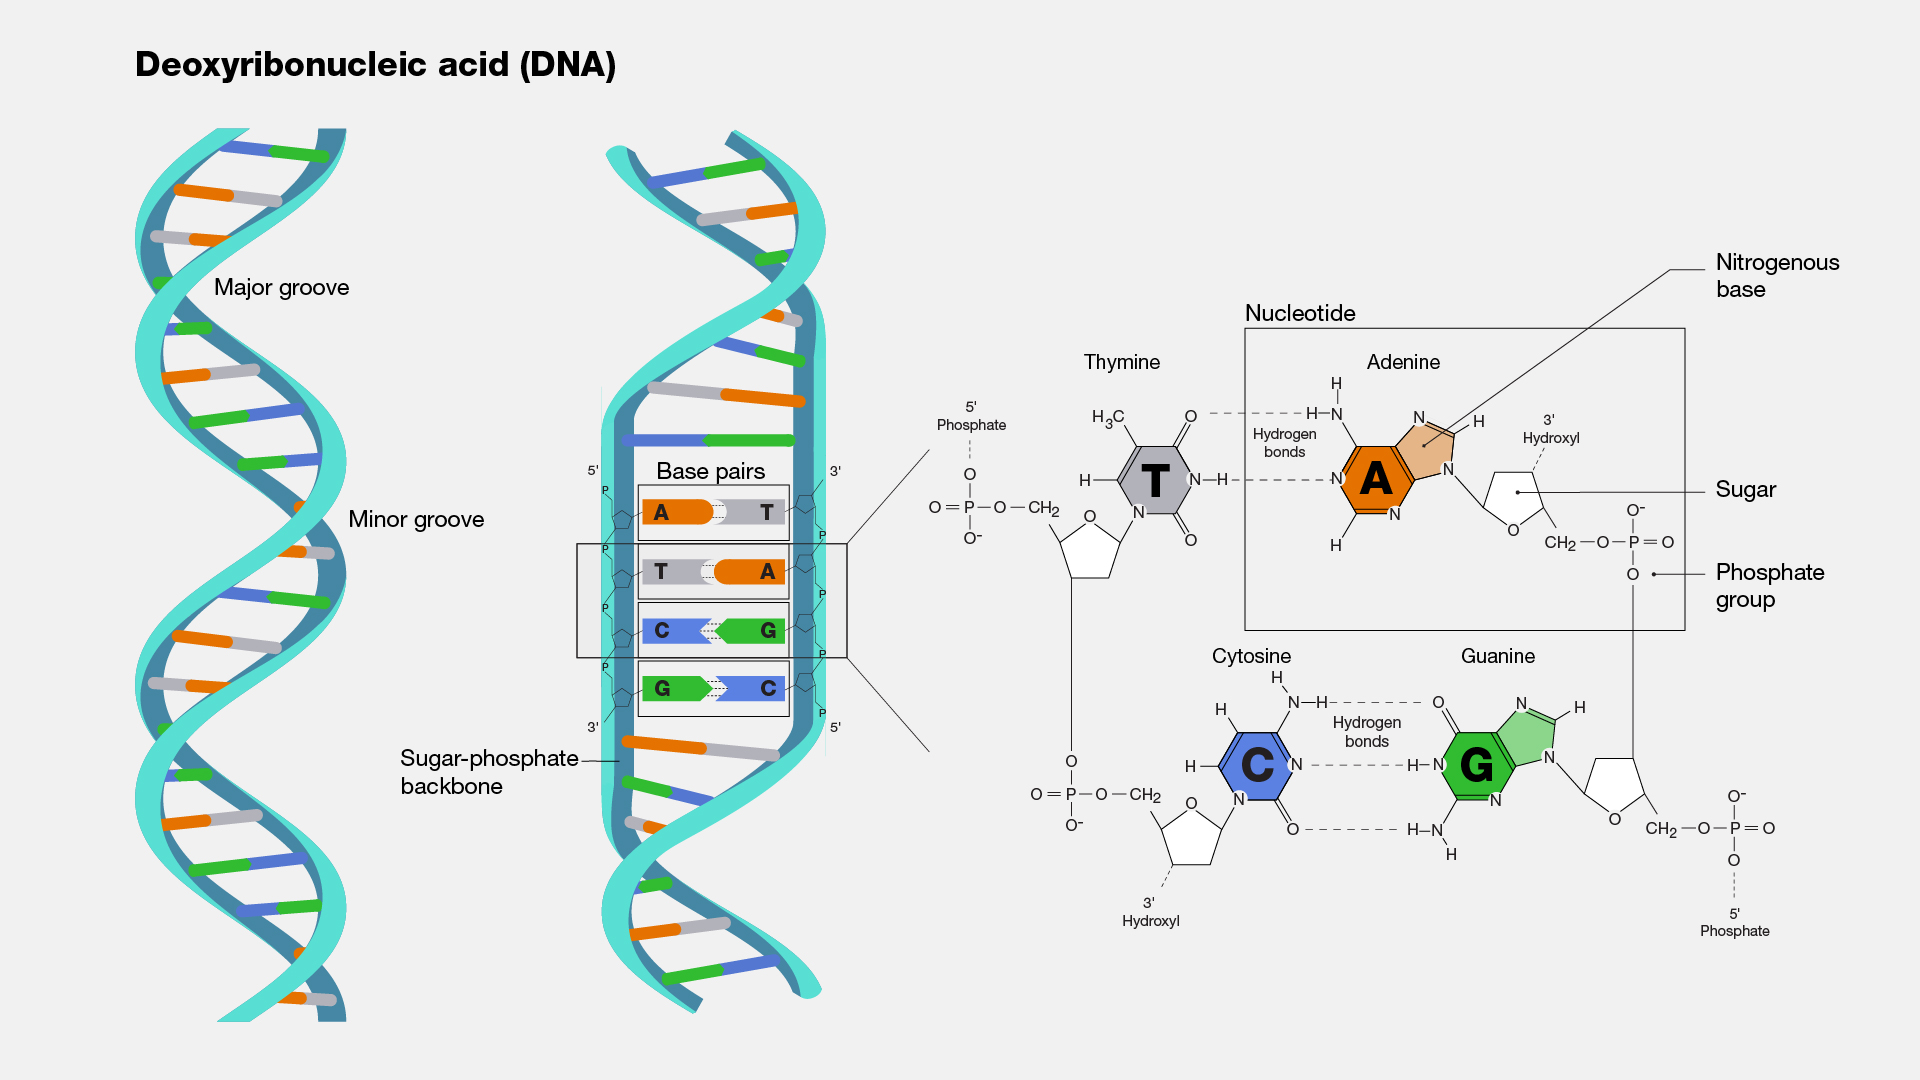
\includegraphics[width=0.6\textwidth]{dna.jpg}
  \caption{Structure of the \gls{dna} double helix}
  \label{fig:dna}
\end{figure}

The functional units of \gls{dna} are called genes, which are discrete
sequences that contain the instructions for producing proteins. However,
\gls{dna} itself cannot participate directly in protein synthesis. Instead, a
process called transcription is used to copy the information from a gene to a
\gls{rna} molecule as seen in \textcite{basic_biology_NCBI2002}. Unlike
\gls{dna}, \gls{rna} is single-stranded and uses uracil (U) instead of thymine
as one of its bases.

Among the various types of \gls{rna}, the best known is messenger \gls{rna}
(mRNA), which serves as an intermediary between genes and proteins. During
transcription, an mRNA molecule is synthesized as a complementary copy of a
gene, and this mRNA carries the genetic message from the \gls{dna} in the
nucleus to the ribosomes in the cytoplasm, where protein synthesis occurs. This
process, known as translation, is where the mRNA sequence is read in triplets
(called codons), each of which corresponds to a specific amino acid
\cite{central_dogma_molecular}.

%melhorar estrutura da imagem para ser como no paper
\begin{figure}[h]
  \centering
  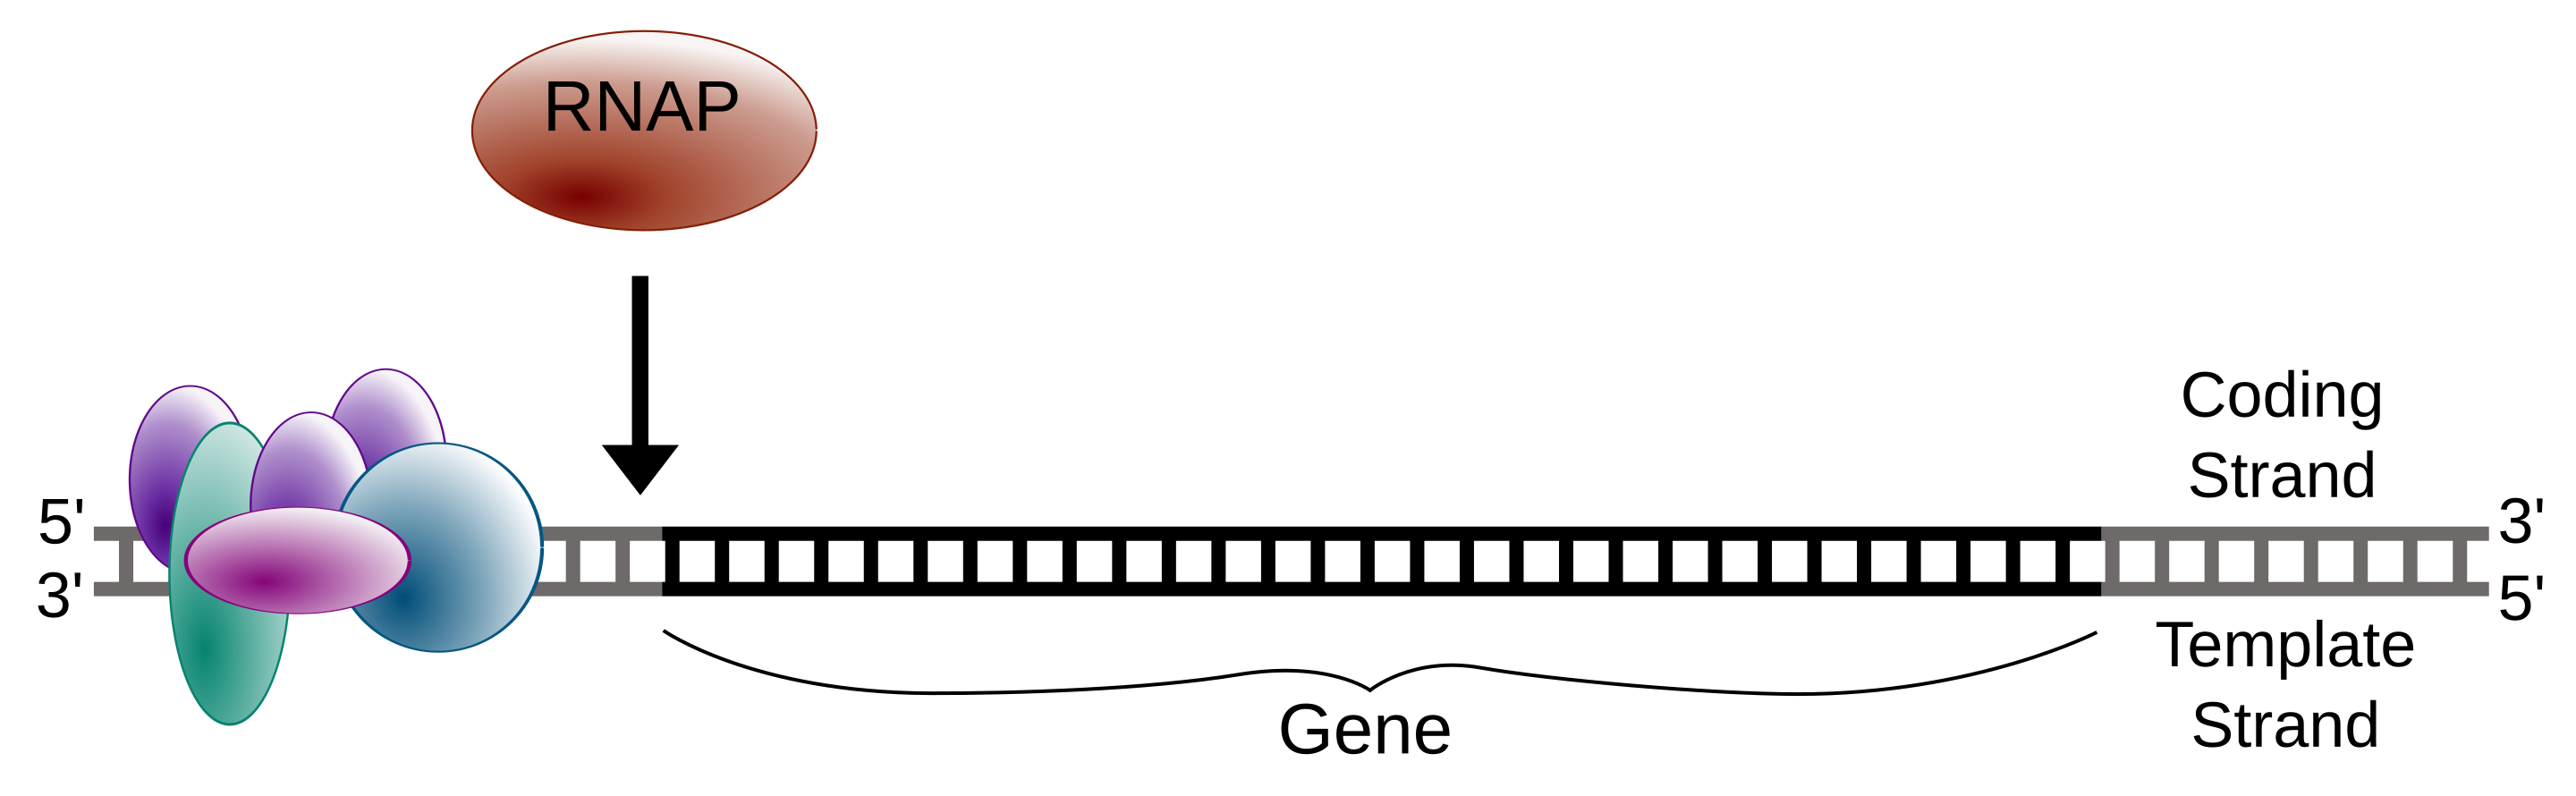
\includegraphics[width=0.3\textwidth]{transcription1.png}
  
\includegraphics[width=0.3\textwidth]{transcription2.png}
  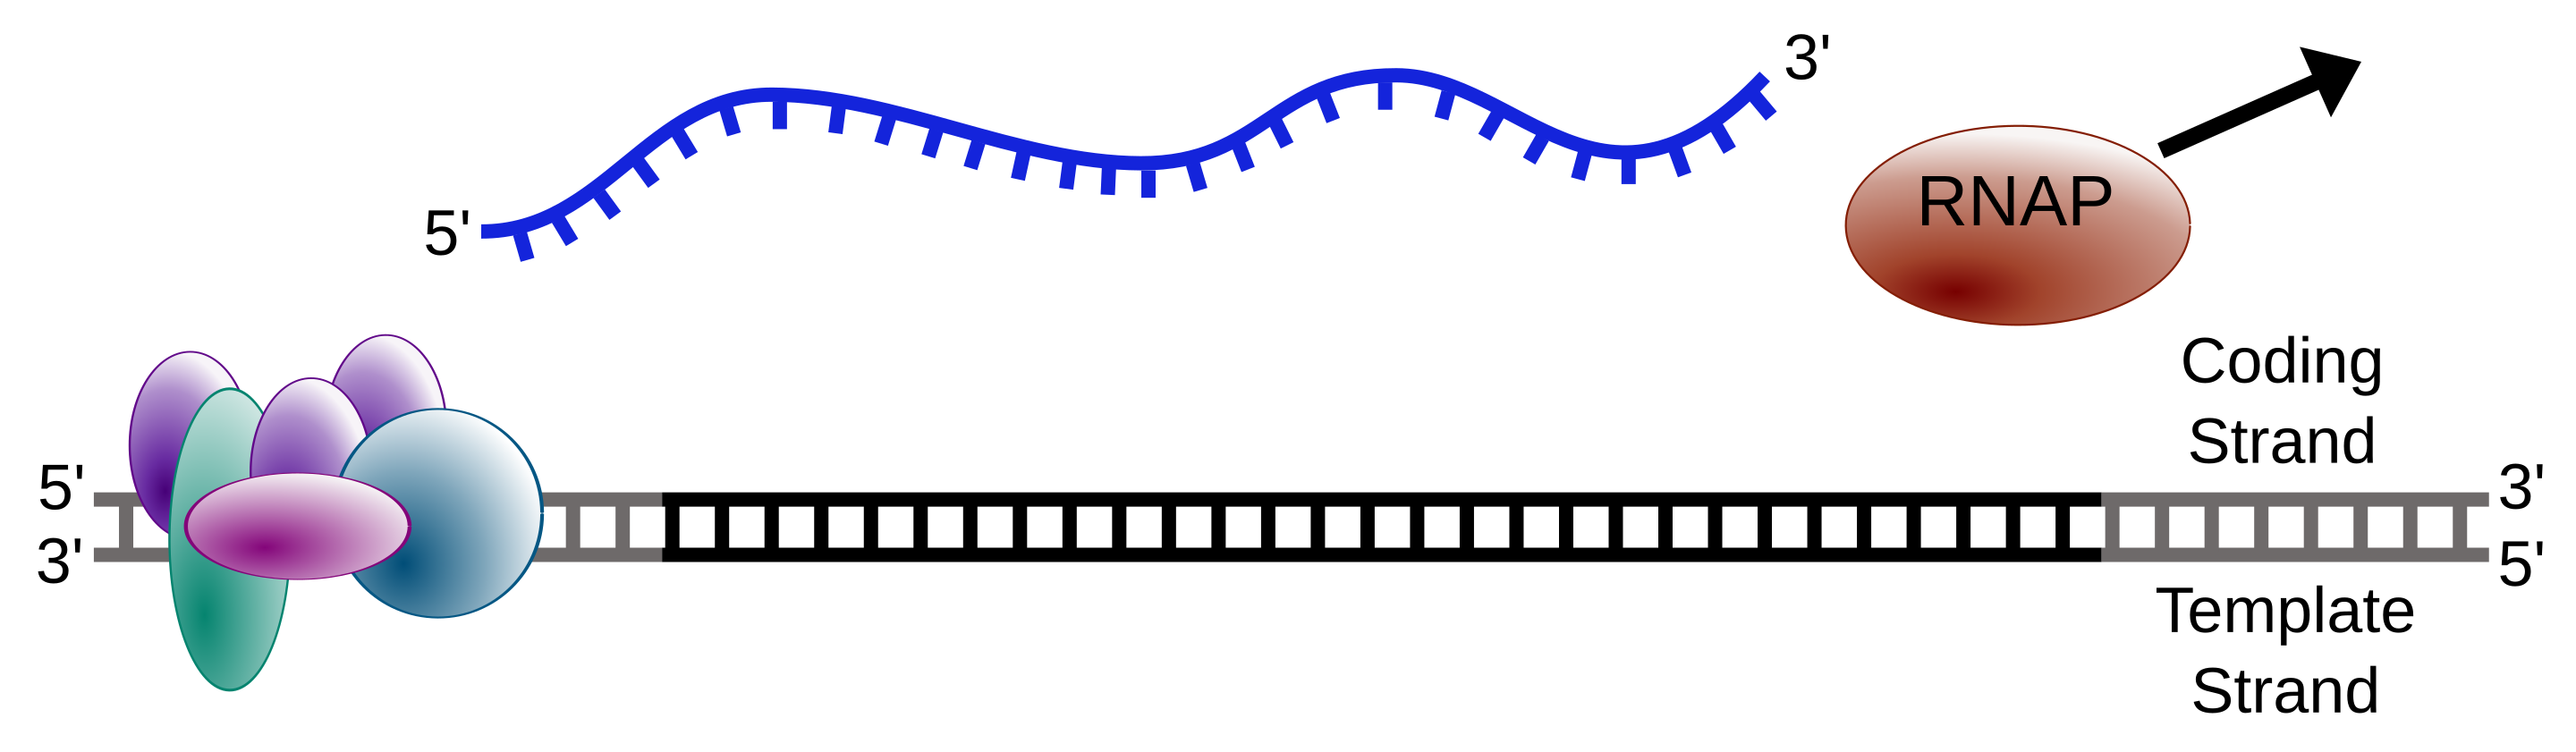
\includegraphics[width=0.3\textwidth]{transcription3.png}
  \caption{Illustration of the transcription mechanism: (a) initiation, (b) elongation, and (c) termination}
  \label{fig:transcription}
\end{figure}

The set of rules by which the nucleotide sequence in messenger \gls{rna} is
translated into a sequence of amino acids is known as the genetic code. This
code is composed of triplets of nucleotides, called codons, where each codon
specifies one of the twenty standard amino acids used in protein synthesis seen
in \textcite{genetic_codeNovozhilov2008O} study.

The genetic code is described as redundant but unambiguous. Redundancy means
that most amino acids are encoded by more than one codon - for example, leucine
is specified by six different codons - which provides a certain degree of
robustness to the system. At the same time, the code is unambiguous because
each codon corresponds to only one amino acid; that is, a given codon does not
encode multiple amino acids \cite{ConceptsBiology_DNA}.

Another fundamental characteristic of the genetic code is its universality.
With very few exceptions, the same codons specify the same amino acids in
virtually all living organisms, from bacteria to humans. This evolutionary
conservation has been fundamental in enabling the development of many molecular
biology tools and biotechnological applications prooved by
\textcite{genetic_codeKoonin2017}.

Although the focus of molecular biology for decades has been on the coding
sequence of the genome - that is, the genes that give rise to proteins - it is
now known that a large part of the human genome is transcribed into \gls{rna}
that does not code for proteins. These non-coding \gls{rna} (ncRNA) molecules
play crucial regulatory roles in controlling gene expression. One of the most
studied groups within this class are \gls{mirna}, which appear to be central
elements in the fine-tuning of the genetic regulation process.

\subsection{MicroRNAs - The Regulators of Gene Expression}
\label{sec:microRNA}
\gls{mirna} are small non-coding \gls{rna} molecules, approximately $20$
to $25$ nucleotides in length, that play a key role in regulating gene
expression at the post-transcriptional level
\cite{regulatory_mecha_mirnaGulyaeva2016,
  first_mirna_Ambros1993,post_transcript_wightman1993}. Instead of encoding
proteins, \gls{mirna} act by controlling the production of proteins from genes.

\begin{figure}[h]
  \centering
  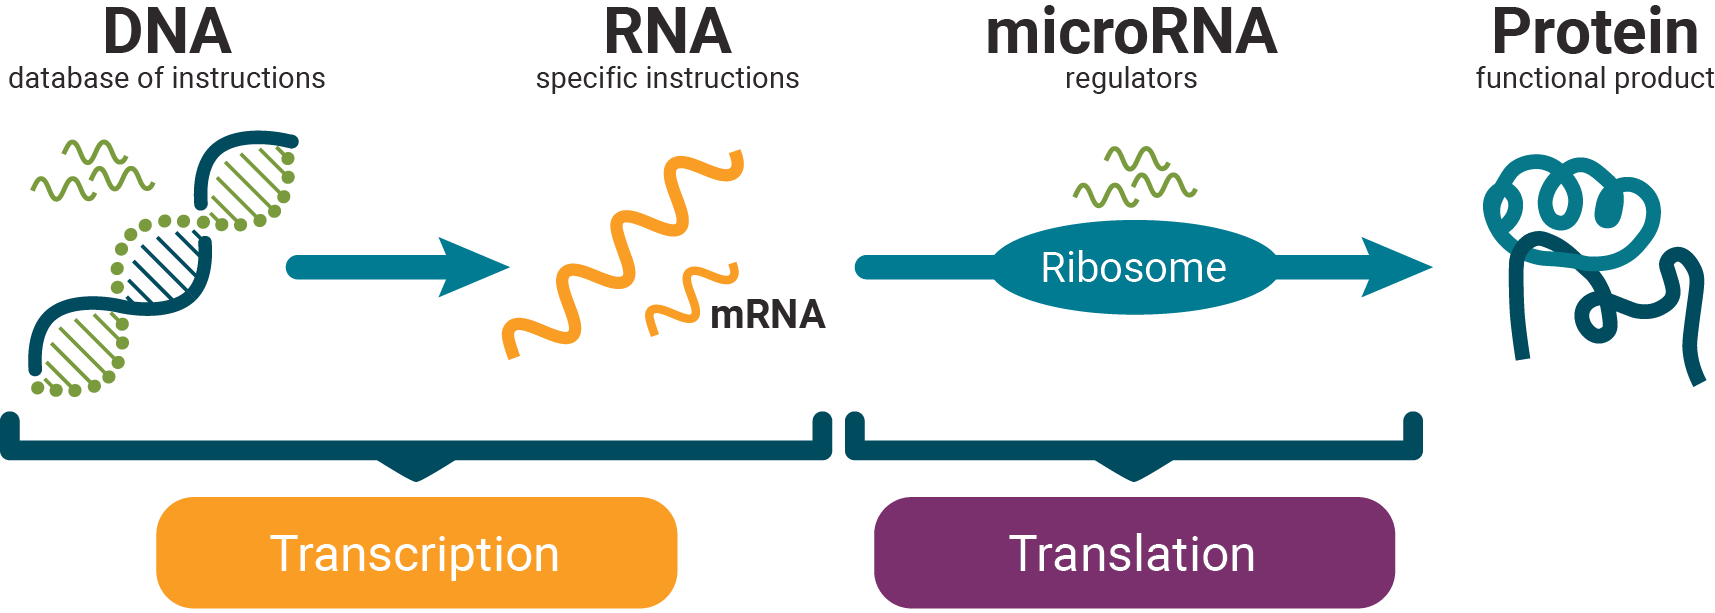
\includegraphics[width=0.8\textwidth]{mirna_process.png}
  \caption{The figure shows the process of gene expression: DNA is transcribed
    into mRNA, which is then translated into protein by the ribosome. \gls{mirna}
    are shown as regulators acting on the mRNA before translation.}
  \label{fig:mirna_mechanism}
\end{figure}

In simple terms, \textbf{\gls{mirna} function as molecular switches that bind
  to messenger \gls{rna} (mRNA) molecules}, blocking their translation into
protein or promoting their degradation. This mechanism depends on the degree of
complementarity between the \gls{mirna} sequence and that of the target mRNA:

\begin{itemize}
  \item When there is high complementarity, the mRNA tends to be degraded;
  \item When complementarity is partial, the \gls{mirna} generally acts by inhibiting
        translation without destroying the mRNA.
\end{itemize}

A study made by \textcite{role_mirna_Calaf2023} demonstrates the high
effienciency of this mechanism of regulation: a \textbf{single \gls{mirna} can
  control dozens to hundreds of different genes}, and it is estimated that more
than $60\%$ of human coding genes are targeted for regulation by \gls{mirna}.

Due to this broad regulatory capacity, \gls{mirna} play a central role in
multiple cellular processes such as proliferation, differentiation, apoptosis,
and stress response. Consequently, changes in \gls{mirna} expression profiles
are associated with several diseases, including cancer, neurodegenerative and
cardiovascular diseases. In an oncological context, \gls{mirna} can act as
oncogenes (promoting tumor growth) or as tumor suppressors, depending on the
biological context and cell type as shown by
\textcite{regulatory_mecha_mirnaGulyaeva2016}.

Due to their specificity, stability, and direct involvement in relevant
molecular mechanisms, \gls{mirna} have been extensively investigated as
promising biomarkers for diagnosis, prognosis, and subtype stratification in
various diseases - including cancer.

\subsection{Cancer - A Complex Disease}
Cancer is a disease characterized by the uncontrolled proliferation of
transformed cells, which can invade neighboring tissues and spread to other
parts of the body through processes such as metastasis. This definition, based
on \textcite{NCI2021,def_of_cancer_Brown2023}, has recently been expanded to
recognize the role of natural selection in the evolution of cancer: it is a
cellular system that continuously evolves, adapting to internal and external
pressures to ensure its survival.

Under normal conditions, the body's cells divide only when necessary, die when
damaged or obsolete, and are replaced by new ones. However, in cancer, this
biological balance is disrupted: abnormal cells gain the ability to multiply
independently of the body's signals and to resist programmed cell death
(apoptosis). These transformed cells become autonomous units that not only
ignore normal growth controls but also interact with the tumor microenvironment
to promote their own survival, using angiogenesis, immune evasion, and other
adaptive mechanisms \cite{def_of_cancer_Brown2023,NCI2021}.

The result is a heterogeneous cell population, subject to natural selection
within the human body. Cells that acquire adaptive advantages (e.g., higher
proliferation rate, drug resistance, or migration ability) tend to prevail,
making cancer a constantly evolving disease \cite{def_of_cancer_Brown2023}.

Although cancer can arise in virtually any tissue, not all cellular changes are
malignant. There are precancerous conditions, such as \textit{hyperplasia or
  dysplasia}, which represent an increase in the number of cells or changes in
their morphology, but which do not yet invade surrounding tissues.

Progression of cancer is a complex process that involves the
\textbf{acquisition of invasive and metastatic capacity - properties that
  distinguish malignant tumors from benign ones}. This process can be silent for
years, until more severe symptoms arise, often related to the invasion of vital
organs.

\subsection{Breast Cancer \& its Subtypes}

Breast cancer is the most commonly diagnosed cancer in women worldwide and is
one of the leading causes of cancer death in developed and developing countries
as seen in \textcite{BreastEpidemiology_Romanowicz2022,
  updatedbca_Hong2022Breast}. It is estimated that \textbf{one in eight women}
will be diagnosed with this disease during their lifetime, although it can also
affect men - albeit with a much lower incidence.

Most breast tumors are originated in the epithelial cells of the ducts or
lobules of the breast, which acquire malignant properties after the
accumulation of genetic and epigenetic changes. These events alter the normal
control of cell proliferation, differentiation, and apoptosis, allowing for
unregulated tumor growth \cite{origins_and_evolution_bca_Polyak2007}.

\begin{figure}
  \centering
  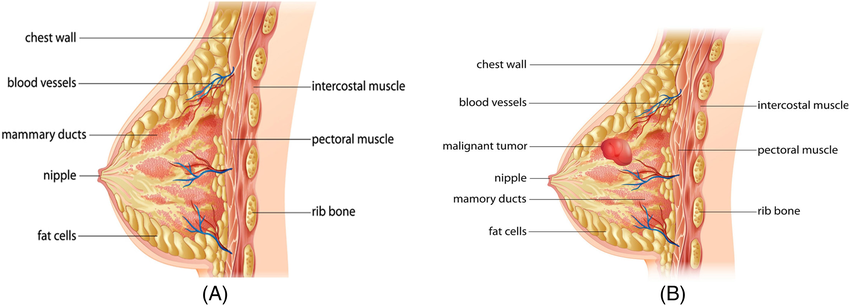
\includegraphics[width=0.8\textwidth]{bca_anatomy.png}
  \caption{In (A) we have a normal breast tissue, while in (B) we can see
    the presence of a malignant tumor \cite{bca_anatomy_figure_Muthu2020}.}
  \label{fig:breast_cancer_anatomy}
\end{figure}

The development of the disease is associated with a set of well-established
risk factors, which include:
\begin{itemize}
  \item Age and family history of the disease;
  \item Hereditary genetic mutations, especially in the \textit{BRCA1} and
        \textit{BRCA2} genes;
  \item Prolonged exposure to endogenous or exogenous hormones (e.g., early menarche,
        late menopause, hormone therapy);
  \item Environmental and behavioral factors, such as obesity, physical inactivity,
        alcohol consumption, and a diet rich in saturated fats
        \cite{BreastEpidemiology_Romanowicz2022,clinical_implication_bca_Adamo2015}.
\end{itemize}

From a molecular and clinical point of view, \textbf{\gls{bc} is highly
  heterogeneous}. Each tumor may have unique combinations of genetic alterations,
signaling pathways, and gene expression profiles, which are reflected in
different clinical behaviors, degrees of aggressiveness, and response to
treatment
\cite{origins_and_evolution_bca_Polyak2007,diff_bca_usa_Howlader2018}.

Early detection is crucial for prognosis. When diagnosed in its early stages,
\gls{bc} has survival rates of over $90\%$. However, in more advanced stages,
especially when metastases appear, controlling the disease becomes
substantially more difficult and the therapeutic goal shifts from curative to
palliative \cite{updatedbca_Hong2022Breast,clinical_implication_bca_Adamo2015}.

The therapeutic approach is typically multimodal, combining surgery,
radiotherapy, chemotherapy, hormone therapy, and targeted or biological
therapies, depending on the characteristics of the tumor and the patient's
general condition. The most significant advance in the last decade has been the
transition from a uniform model to a personalized treatment approach, tailored
to the molecular subtype and individual risk as studied by
\textcite{BreastEpidemiology_Romanowicz2022}.

In addition, a study made by \textcite{origins_and_evolution_bca_Polyak2007}
recognized that breast tumors are not static entities. Due to phenomena of
intra-tumor heterogeneity and clonal evolution, tumors adapt to the selective
pressure of treatments, often leading to the development of therapeutic
resistance and disease progression.

Given the molecular complexity and clinical diversity of breast tumors, it was
established in the papers
\textcite{clinical_implication_bca_Adamo2015,bc_subtypes_Prat2015Clinical} that
\gls{bc} is not a single disease but rather a collection of biologically
distinct entities that arise from a common anatomical site. This heterogeneity
is reflected in major differences in tumor progression, metastatic behavior,
response to therapy, and long-term prognosis.

To better capture this complexity and inform clinical decision-making,
researchers from various studies, such as
\textcite{bc_molecular_Perou2000,bc_subtypes_Prat2015Clinical}, have developed
a molecular classification system that subdivides breast tumors into intrinsic
subtypes. These subtypes are defined based on the expression status of three
key biomarkers: \textbf{estrogen receptor (ER)}, \textbf{progesterone receptor
  (PR)}, and \textbf{human epidermal growth factor receptor 2 (HER2)} as well as
other proliferation indices (e.g., Ki-67) and gene expression patterns. This
classification underpins modern precision oncology approaches and has profound
implications for therapy and prognosis.

As shown in the table \ref{tab:bc_subtypes_summary}, \gls{bc} can be classified
into four main intrinsic subtypes based on the expression of these biomarkers
and other molecular characteristics:

%%% REMOVER O h para !t no final1!!!!!!asdonasodniasoindaosindoi
\renewcommand{\arraystretch}{1.3}
\begin{table}[h]
  \centering
  \small
  \caption{Summary of intrinsic \gls{bc} subtypes and typical characteristics of each one.\newline\textit{References:} \cite{clinical_implication_bca_Adamo2015}, \cite{diff_bca_usa_Howlader2018}, \cite{bc_subtypes_Prat2015Clinical}, \cite{updatedbca_Hong2022Breast}, \cite{tnbc_therapies_Mahalingam2020The}.}
  \label{tab:bc_subtypes_summary}
  \begin{tabularx}{\textwidth}{l l l l X}
    \toprule
    \textbf{Subtype}  & \textbf{Receptors / HER2} & \textbf{Prolif.} & \textbf{Prognosis} & \textbf{Treatment}          \\
    \midrule
    Luminal A         & ER+/PR+, HER2−            & Low              & Favorable          & Endocrine only              \\
    \midrule
    Luminal B         & ER+, PR↓, HER2±           & High             & Intermediate       & Hormone ± Chemo ± Anti-HER2 \\
    \midrule
    HER2-enriched     & HER2+, ER−, PR−           & High             & Improved           & Anti-HER2 + Chemo           \\
    \midrule
    Basal-like / TNBC & ER−, PR−, HER2−           & High             & Poor               & Chemo; ± PARP/IO (selected) \\

    \bottomrule
  \end{tabularx}

  \vspace{1ex}
  \raggedright
  \footnotesize
  \textit{Acronyms:} Chemo = Chemotherapy , IO = Immunotherapy .
\end{table}

Recent evidence by
\textcite{intratumor_heterogeneity_Yeo2017,origins_and_evolution_bca_Polyak2007}
suggests that multiple subtypes can coexist within the same tumor (a phenomenon
called intra-tumor heterogeneity). This complexity contributes to therapeutic
resistance and disease progression.

\subsection{Nucleic acids as gene therapies}
\label{sec:nucleic_acids_gene_therapies}
% Now that we have a better understanding of limitations that most of cancer treatments 
% have, \gls{mirna} have emerged as a promising tool in the field of cancer
% research and treatment. 

% Considering them as the "natural regulators" of the human body, we can leverage 
% that regulating mechanism and use it to 

\newpage
\section{Related work}

This section will present a critical review of computational approaches
developed to date to explore the potential of \gls{mirna} as biomarkers in the
context of oncology, covering both \gls{bc} and other malignant neoplasms. The
contributions of \gls{ml} and \gls{dl} models applied to the task of
classifying different cancer subtypes will also be analyzed, with a special
focus on methodologies that integrate molecular data with data from other
nature, like clinical characteristics for example.

\gls{ml}, a branch of \gls{ai}, involves
developing computational models that learn from data to make predictions or
decisions. These models are typically trained using either supervised
learning, where the target outcomes are known and used during training, or
unsupervised learning, in which no explicit labels or outcome variables are
provided. In both paradigms, the goal is to uncover meaningful patterns in the
data that can be used to generate predictive insights, such as detecting the
presence of cancer, estimating survival probabilities, or stratifying patients
into risk categories. \gls{ml} techniques are particularly valuable when dealing with
unstructured or complex clinical datasets, as is often the case in oncology.

In recent years, the application of \gls{ml} algorithms to the field of
biomedicine has led to significant advances in the analysis of complex and
high-dimensional data, including the expression of \gls{mirna} in cancer
\cite{role_of_ai_giger2021}. In this context, several studies have explored the
use of computational models for the classification of tumor subtypes and/or the
identification of discriminative biomarkers, with promising results but also
with important limitations.

In this context, we will review and analyze scientific works that have
leveraged \gls{ml} algorithms in contexts similar to the stratification of
\gls{bc} subtypes based on \gls{mirna} expression profiles, complementing them
with data of other types (multi-omics data). For each study, it will be
important to define the specific work in question so that we can analyze the
methodology, algorithms used, and results obtained, all based on the specific
context of the research in question, in order to capture and consolidate a
ground on which we can work. At the end of the review, we will discuss how
these contributions inform and substantiate the methodological choices made in
the present work, justifying, whenever possible, the algorithmic and
experimental choices based on the available scientific evidence.

\subsection{Leveraging \gls{ai} models for cancer classification}
% HERE: começar com cancer classification em geral -> depois falar de 
% Papers a usar: 4, 10 , 11, 12 ( estes dois últimos são com imagens, mas podemos abordar)

The classification of different types of cancer using computational models has
been one of the most explored areas within the application of \gls{ai} to
medicine. Let's take a look at the work of
\textcite{ai_in_dermacancer_esteva2017}, a remarkable advance in this “new”
relationship between computers and dermatology, where deep neural networks
(Figure \ref{fig:DNN}) have demonstrated capabilities comparable to those of
human experts in the diagnosis of malignant skin lesions.

\begin{figure}[htbp]
  \centering
  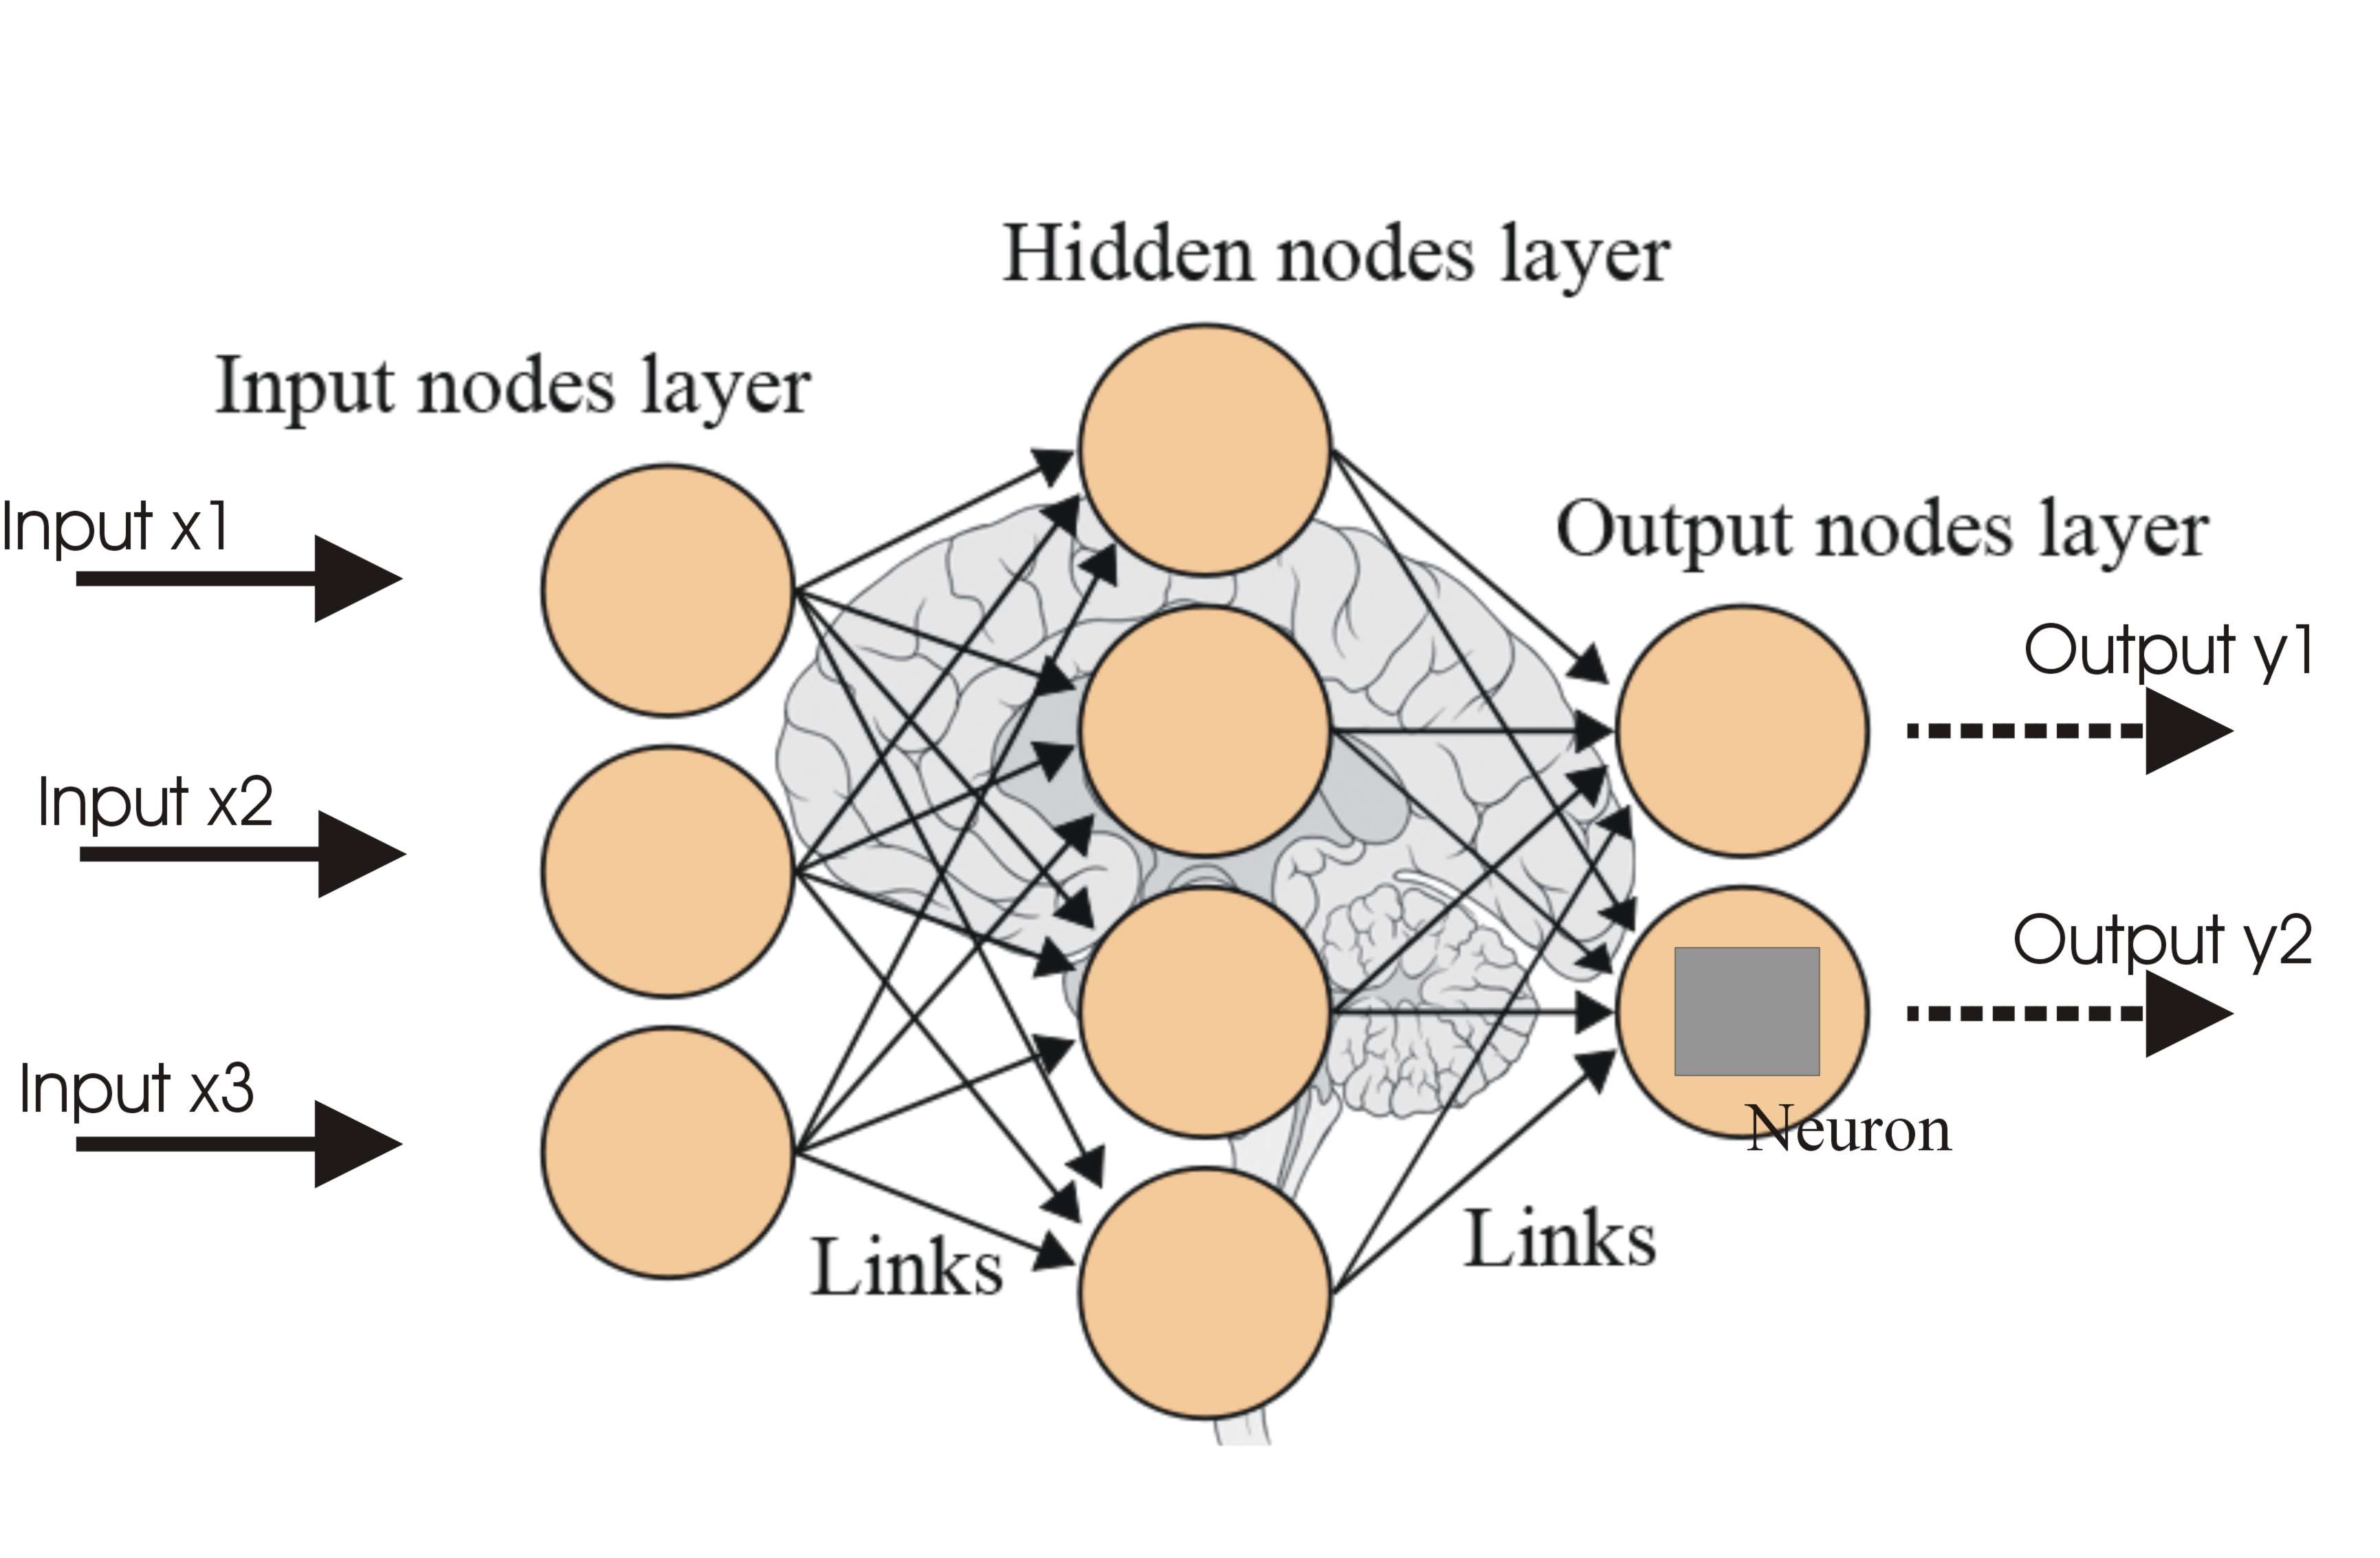
\includegraphics[width=0.7\textwidth]{/Users/JoseRomano/Documents/Tese/bca-thesis/Chapters/Figures/NN.png}
  \caption{Structure of an deep neural network (DNNs). It shows the input, hidden, and output layers, with connections between neurons responsible for processing information \cite{analyticsvidhya_image}.}
  \label{fig:DNN}
\end{figure}

This work was made possible by the use of an architecture based on
convolutional neural networks (CNNs) - a type of DNN that is particularly
effective in image processing (Figure \ref{fig:CNN_derma}). CNNs work by
applying convolutional filters that extract visual patterns at different levels
of complexity, allowing the model to identify relevant features directly from
the image pixels, without the need for specialized preprocessing
\cite{CNN_Albawi2017}.

\begin{figure}[htbp]
  \centering
  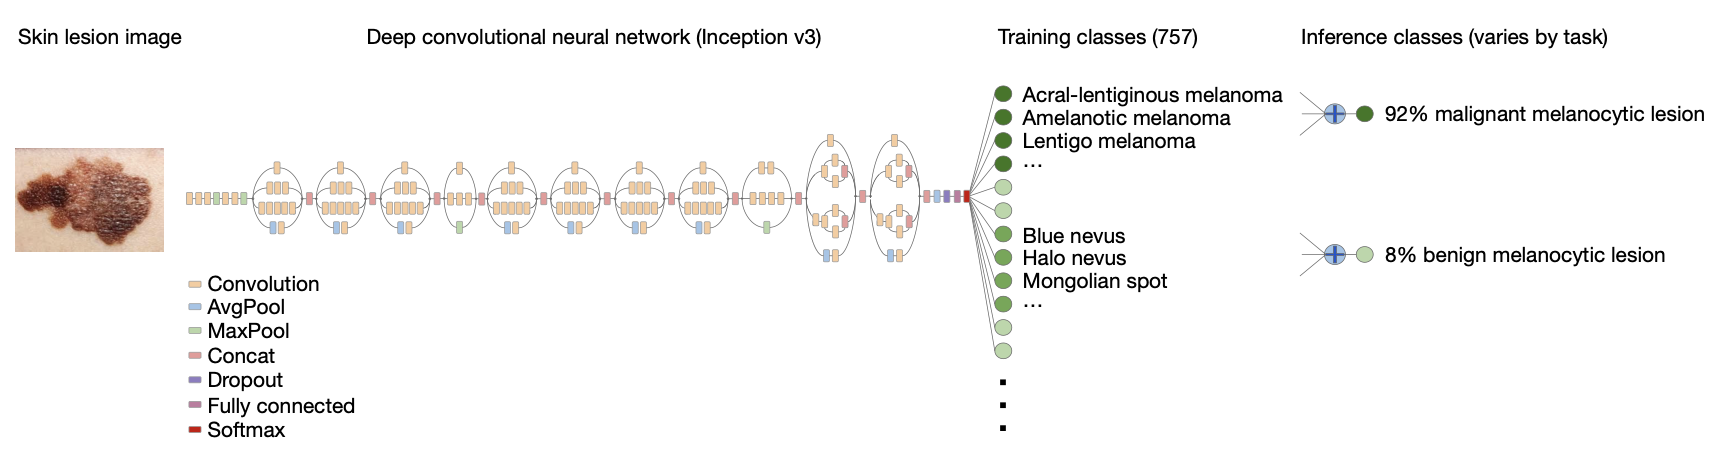
\includegraphics[width=1.0\textwidth]{/Users/JoseRomano/Documents/Tese/bca-thesis/Chapters/Figures/CNN_derma.png}
  \caption{Schematic of the CNN used by \textcite{ai_in_dermacancer_esteva2017} with Inception v3 architecture, adapted to classify skin lesions based on clinical images. The network generates a probability distribution over clinical classes, based on a structured medical taxonomy.}
  \label{fig:CNN_derma}
\end{figure}

The biggest problem with this methodology is that these architectures require a
large number of cases (positive and negative) in order to learn the necessary
patterns. In this case, 129{,}450 clinical images covering more than 2{,}000
different diseases were used. Some factors that determined the good results of
this model were:

\begin{enumerate}
  \item The photographic variability of the samples on which it was trained, since they
        covered not only images taken with mobile phones, but also dermoscopy images;

  \item The manipulation of images during training, enlarging and inverting them to
        increase the adaptability and robustness of the model;

  \item The use of a structured medical taxonomy (Figure \ref{fig:taxonomy}), built on
        clinical and visual criteria, which allowed for the organization of more than
        2{,}000 diseases into a hierarchy of 757 fine-grained training classes, such as
        \textit{acrolentiginous melanoma} and \textit{amelanotic melanoma}.
\end{enumerate}

\begin{figure}[htbp]
  \centering
  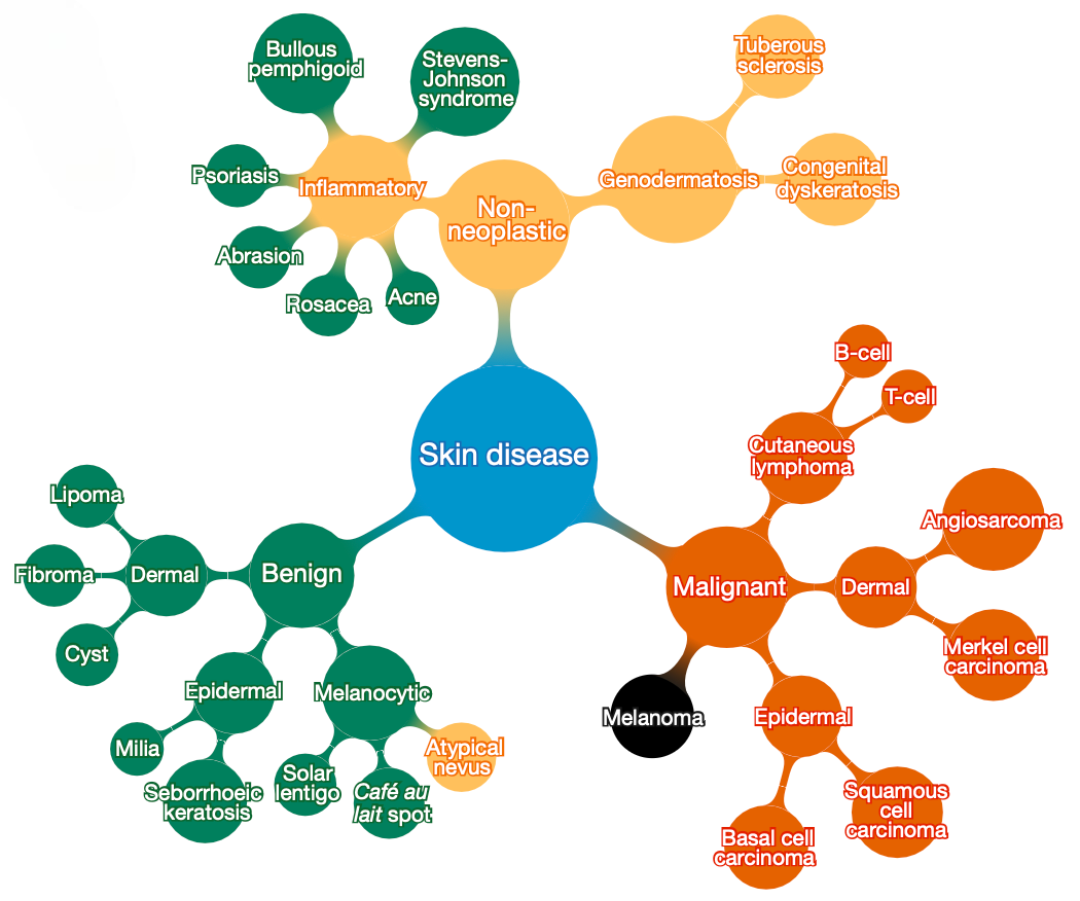
\includegraphics[width=0.5\textwidth]{/Users/JoseRomano/Documents/Tese/bca-thesis/Chapters/Figures/taxonomy.png}
  \caption{A subset of the hierarchical taxonomy developed in the study by \textcite{ai_in_dermacancer_esteva2017}, with diseases organized by clinical and visual similarity into three major groups: benign, malignant, and non-neoplastic.}
  \label{fig:taxonomy}
\end{figure}

The result? A computational model that not only achieved performance comparable
to that of certified dermatologists, but in several scenarios even demonstrated
superiority over average human performance, verifiably by this confusion matrix
(Figure \ref{fig:conf-matrix-docs}). The trained convolutional neural network
was able to classify two critical clinical cases with high accuracy:
keratinocytic carcinomas versus benign seborrheic keratoses, and malignant
melanomas versus benign nevi. In these binary scenarios, it obtained areas
under the curve (\textit{AUC}) of 0.96 and 0.94, respectively (Figure
\ref{fig:AUC_derma_total_dnn_model}) - values higher than those obtained by
dermatologists in the same tasks. \textit{AUC} is a metric that quantifies a
model's ability to distinguish between classes, with values close to 1
indicating excellent performance.

\begin{figure}[htbp]
  \centering
  \begin{subfigure}[b]{0.45\textwidth}
    \centering
    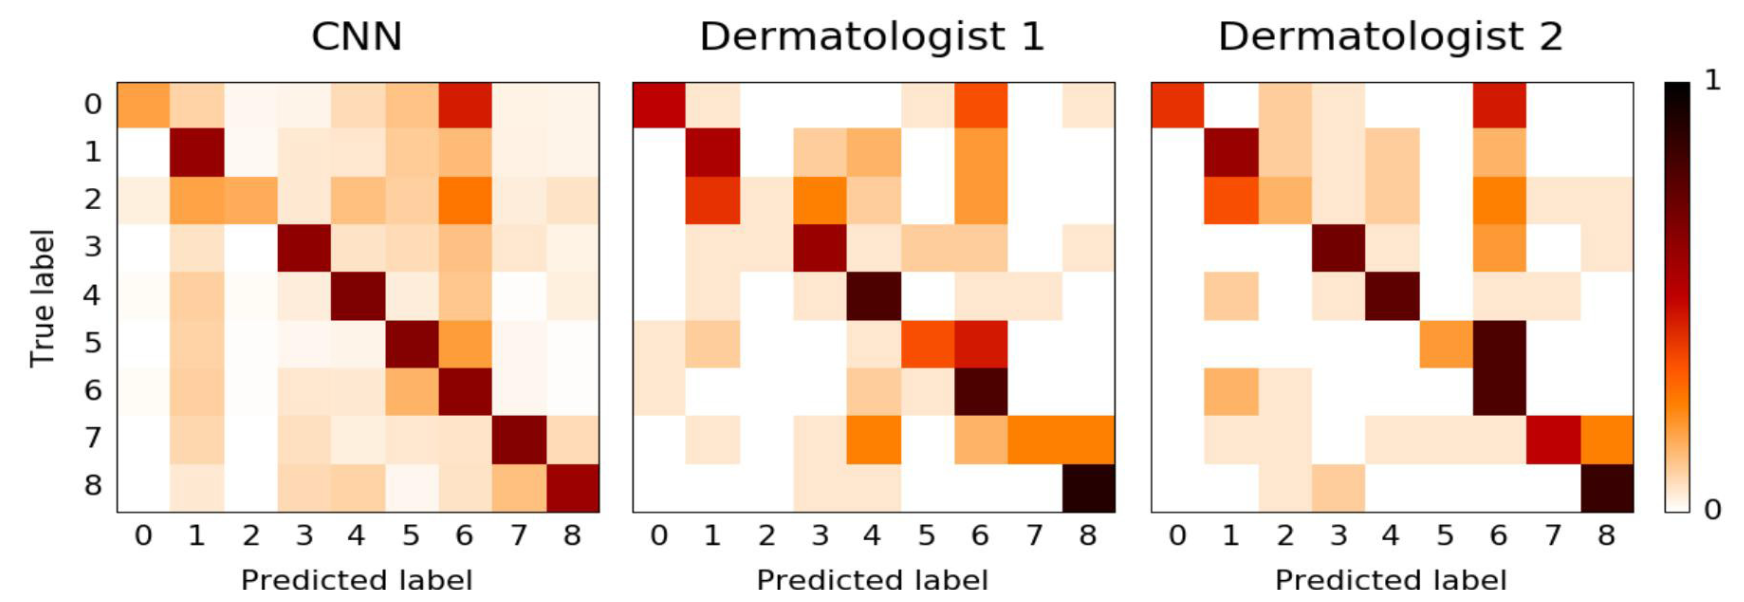
\includegraphics[width=\textwidth]{/Users/JoseRomano/Documents/Tese/bca-thesis/Chapters/Figures/conf-matrix-docs.png}
    %\caption{(a)}
    \label{fig:conf-matrix-docs}
  \end{subfigure}
  \hfill
  \begin{subfigure}[b]{0.45\textwidth}
    \centering
    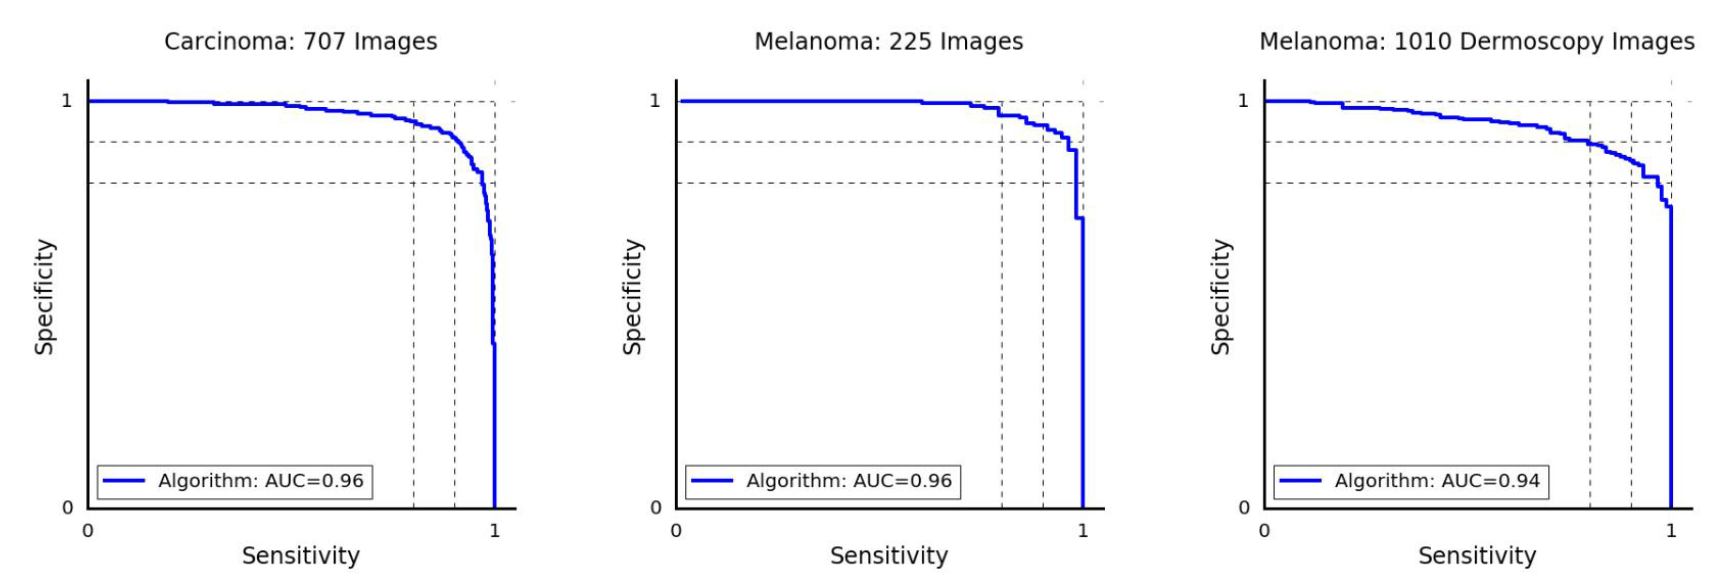
\includegraphics[width=\textwidth]{/Users/JoseRomano/Documents/Tese/bca-thesis/Chapters/Figures/AUC_derma_2.png}
    %\caption{(b)}
    \label{fig:AUC_dnn_model}
  \end{subfigure}
  \caption{Performance evaluation of the convolutional neural network (CNN) in skin lesion classification. (a) Confusion matrices of CNN and two dermatologists. The concentration on the diagonal indicates correct classifications; CNN shows less dispersion and better overall performance \cite{ai_in_dermacancer_esteva2017}. (b) Reliability of the CNN demonstrated by \textit{AUC} curves on a larger, independent dataset \cite{ai_in_dermacancer_esteva2017}.}
  \label{fig:AUC_derma_total}
\end{figure}

Furthermore, in more complex scenarios with multiple classes (three and nine
disease categories), the model maintained \textbf{remarkable levels of
  accuracy} (72.1\% and 55.4\%), surpassing or equaling human experts. The
robustness of the methodology, that is, its ability to maintain performance
under different conditions or test data, was also confirmed in larger test
sets, where the network's performance remained stable, with \textbf{minimal
  variations in evaluation metrics}. From a technical standpoint, it was an
efficient, scalable system with \textbf{potential for application in mobile
  devices}, which gives it relevant clinical applicability, especially in
contexts with limited access to specialists.

Internal analyses further reinforced confidence in the model, showing that it
learned consistent clinical representations: the network tended to
\textbf{group diseases with similar visual characteristics} (Figure
\ref{fig:tsne_derma}) and focused its attention on the damaged areas of the
images, ignoring irrelevant regions such as background or healthy skin -
promising evidence of \textit{automated clinical focus} with real practical
utility.

\begin{figure} [h]
  \centering
  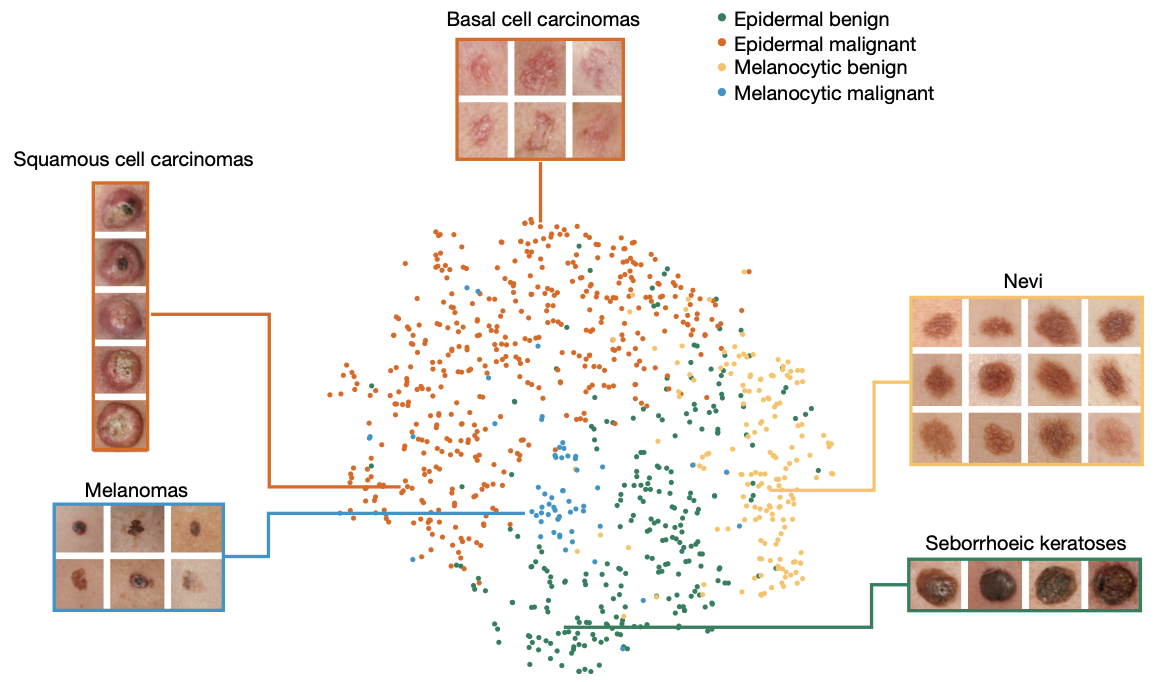
\includegraphics[width=0.5\textwidth]{/Users/JoseRomano/Documents/Tese/bca-thesis/Chapters/Figures/t_sne_derma.png}
  \caption{t-SNE projection of the internal representations of the last hidden layer of the CNN \cite{ai_in_dermacancer_esteva2017}. The different classes of lesions are grouped into distinct clouds, revealing the model's ability to extract relevant discriminative features.}
  \label{fig:tsne_derma}
\end{figure}

\noindent\rule{\linewidth}{0.4pt}

The effectiveness demonstrated in the previous project shows the magnitude of
the benefits that \gls{ai} can bring to the world of medicine, helping doctors
diagnose and stratify diseases with an accuracy that, in some cases, surpasses
that of human specialists. This capability is not limited to imaging data: it
also extends to the field of molecular data and dermatology, as demonstrated by
the study by \textcite{bca_subtypes_with_ml_Wu_2021}, which applies machine
learning algorithms to the task of classifying \gls{bc} subtypes (in this case,
the goal was to distinguish between Triple Negative, or basal-like, and
non-Triple Negative tumors, since TNBC is the most deadly cancer with the most
difficult prognosis, as we saw in the table).

In the study by \textcite{bca_subtypes_with_ml_Wu_2021}, when working with gene
expression data from thousands of patients, additional challenges arise related
to the high dimensionality of the data, requiring robust feature selection
methods and predictive models capable of dealing with complex and often
non-linear correlations. This type of study brings us closer not only to the
context of this thesis, but also to the type of challenges we will encounter
and how we can take advantage of the methodologies used in this paper to
achieve good results. From all the algorithms that were tested, Support Vector
Machine (\textit{SVM}) stood out for its performance. This approach allowed the
authors to achieve high levels of accuracy, sensitivity, and specificity,
demonstrating the potential of \gls{ai} in classifying \gls{bc} subtypes based
on genomic information. The type of information for this study was the
RNA-Sequence (RNA-Seq) profiles made available by The Cancer Genome Atlas
(TCGA), a public database containing thousands of tumor samples characterized
at the genomic level. This dataset, after pre processing, had 934 tumor samples
and over 57{,}000 genes per sample, a typical high-dimensionality scenario
where the number of variables far exceeds the number of observations, and
considering that not all of them are necessary or have a great impact,
\textbf{differential expression analysis was applied} - a bioinformatics
technique used to detect which genes are significantly more or less expressed
between different conditions - resulting in the selection of 5{,}502
differentially expressed genes, which served as input for the predictive models
(a large reduction of over 50{,}000 genes). This step corresponds to feature
selection, which is essential in problems where there is a high risk of
\textit{overfitting} - that is, when the model memorizes the training data but
fails to generalize to new examples.

\begin{figure} [h]
  \centering
  
\includegraphics[width=1.0\textwidth]{/Users/JoseRomano/Documents/Tese/bca-thesis/Chapters/Figures/overfit.png}
  \caption{Examples of underfitting, proper fitting, and overfitting.
    From left to right: the model underfits the data, fits it appropriately, and overfits by capturing noise instead of the underlying pattern \cite{overfiting_ailab_mti_image}.}
  \label{fig:overfitting}
\end{figure}

Now that the dataset had been reduced to a more informative and manageable
subset of features, the authors moved on to the predictive modeling phase. This
is a crucial moment in the \gls{ml} pipeline, where the ability of different
algorithms to learn discriminative patterns present in the data is tested - in
this case, distinguishing between TNBC and non-TNBC tumors based on the
expression levels of selected genes. Several classic supervised learning
algorithms were then evaluated, representing different approaches to the
classification task:

\begin{itemize}
  \label{list:models}
  \item \textbf{K-nearest Neighbors (\textit{kNN})}: classifies new data based on the K nearest neighbors in the feature space \cite{knn_article}.
        \begin{figure} [h]
          \centering
          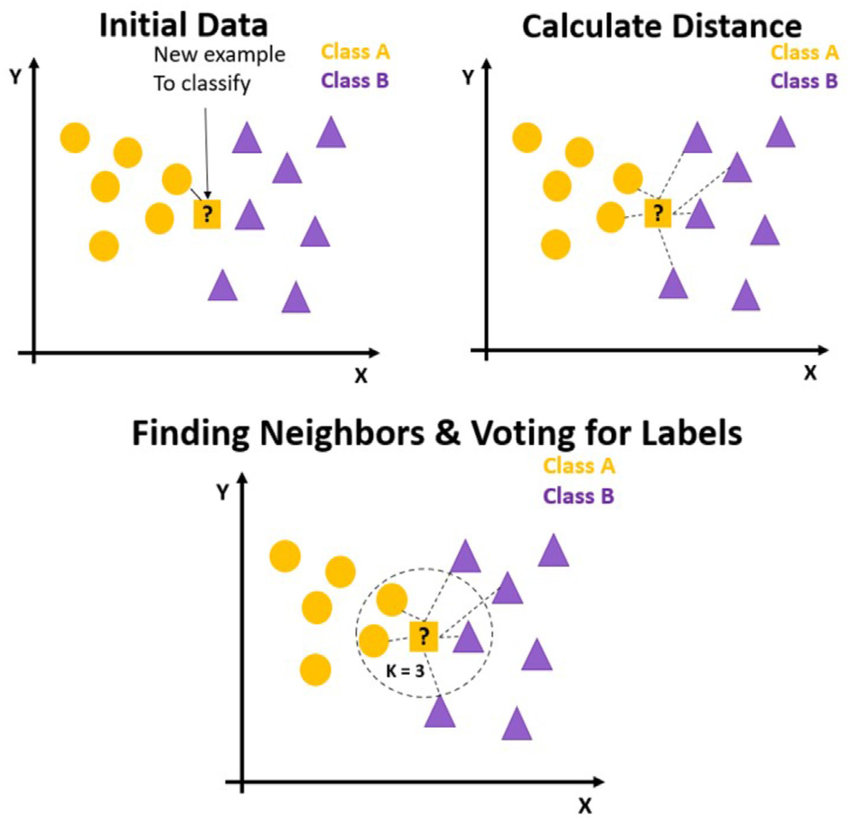
\includegraphics[width=0.45\linewidth]{/Users/JoseRomano/Documents/Tese/bca-thesis/Chapters/Figures/knn-example.jpg}
          \caption{Illustration of the k-Nearest Neighbors (k-NN) classification process. The top-left panel shows the initial labeled data (Class A in yellow, Class B in purple) and a new unlabeled sample (?). The top-right panel demonstrates the calculation of distances from the new sample to all existing points. The bottom panel shows the selection of the k=3 nearest neighbors and class assignment based on majority voting, resulting in the classification of the new sample.}
        \end{figure}

  \item \textbf{Naïve Bayes (\textit{NB})}: uses Bayes' Theorem to estimate the most likely class of a sample, assuming that the input variables are independent of each other \cite{naivebayes_Watson2001}.
        \[
          P(C_k \mid \mathbf{x}) = \frac{P(C_k) \prod_{i=1}^n P(x_i \mid C_k)}{P(\mathbf{x})}
        \]

  \item \textbf{Decision Tree (\textit{DT})}: a model that makes decisions through a hierarchical tree-shaped structure, where each internal node represents a condition on a variable, and each branch represents a possible outcome of that condition. The process continues until it reaches a leaf node, which indicates the final class or value \cite{decision_trees_Jijo2021}.
        \begin{figure} [h]
          \centering
          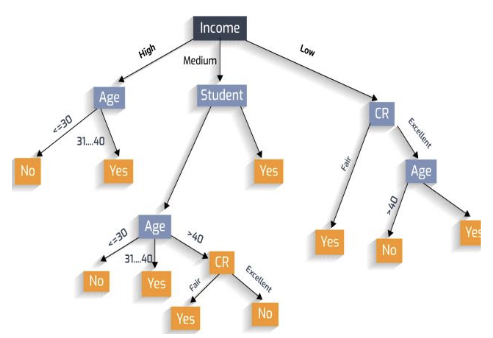
\includegraphics[width=0.45\linewidth]{/Users/JoseRomano/Documents/Tese/bca-thesis/Chapters/Figures/dt-example.png}
          \caption{Example of a Decision Tree for Classification Based on Attributes: Income, Age, Student Status, and Credit Rating (CR). The tree predicts a binary decision outcome (Yes/No) using hierarchical decision rules \cite{decision_trees_Jijo2021Classification}.}
        \end{figure}

  \item \textbf{Support Vector Machine (\textit{SVM})}: This algorithm constructs an optimal hyperplane that best separates samples from different classes. The goal of SVM is to maximize the margin between the two classes for better generalization. Support vectors are the data points that lie closest to the hyperplane and define its position.
        \begin{figure} [h]
          \centering
          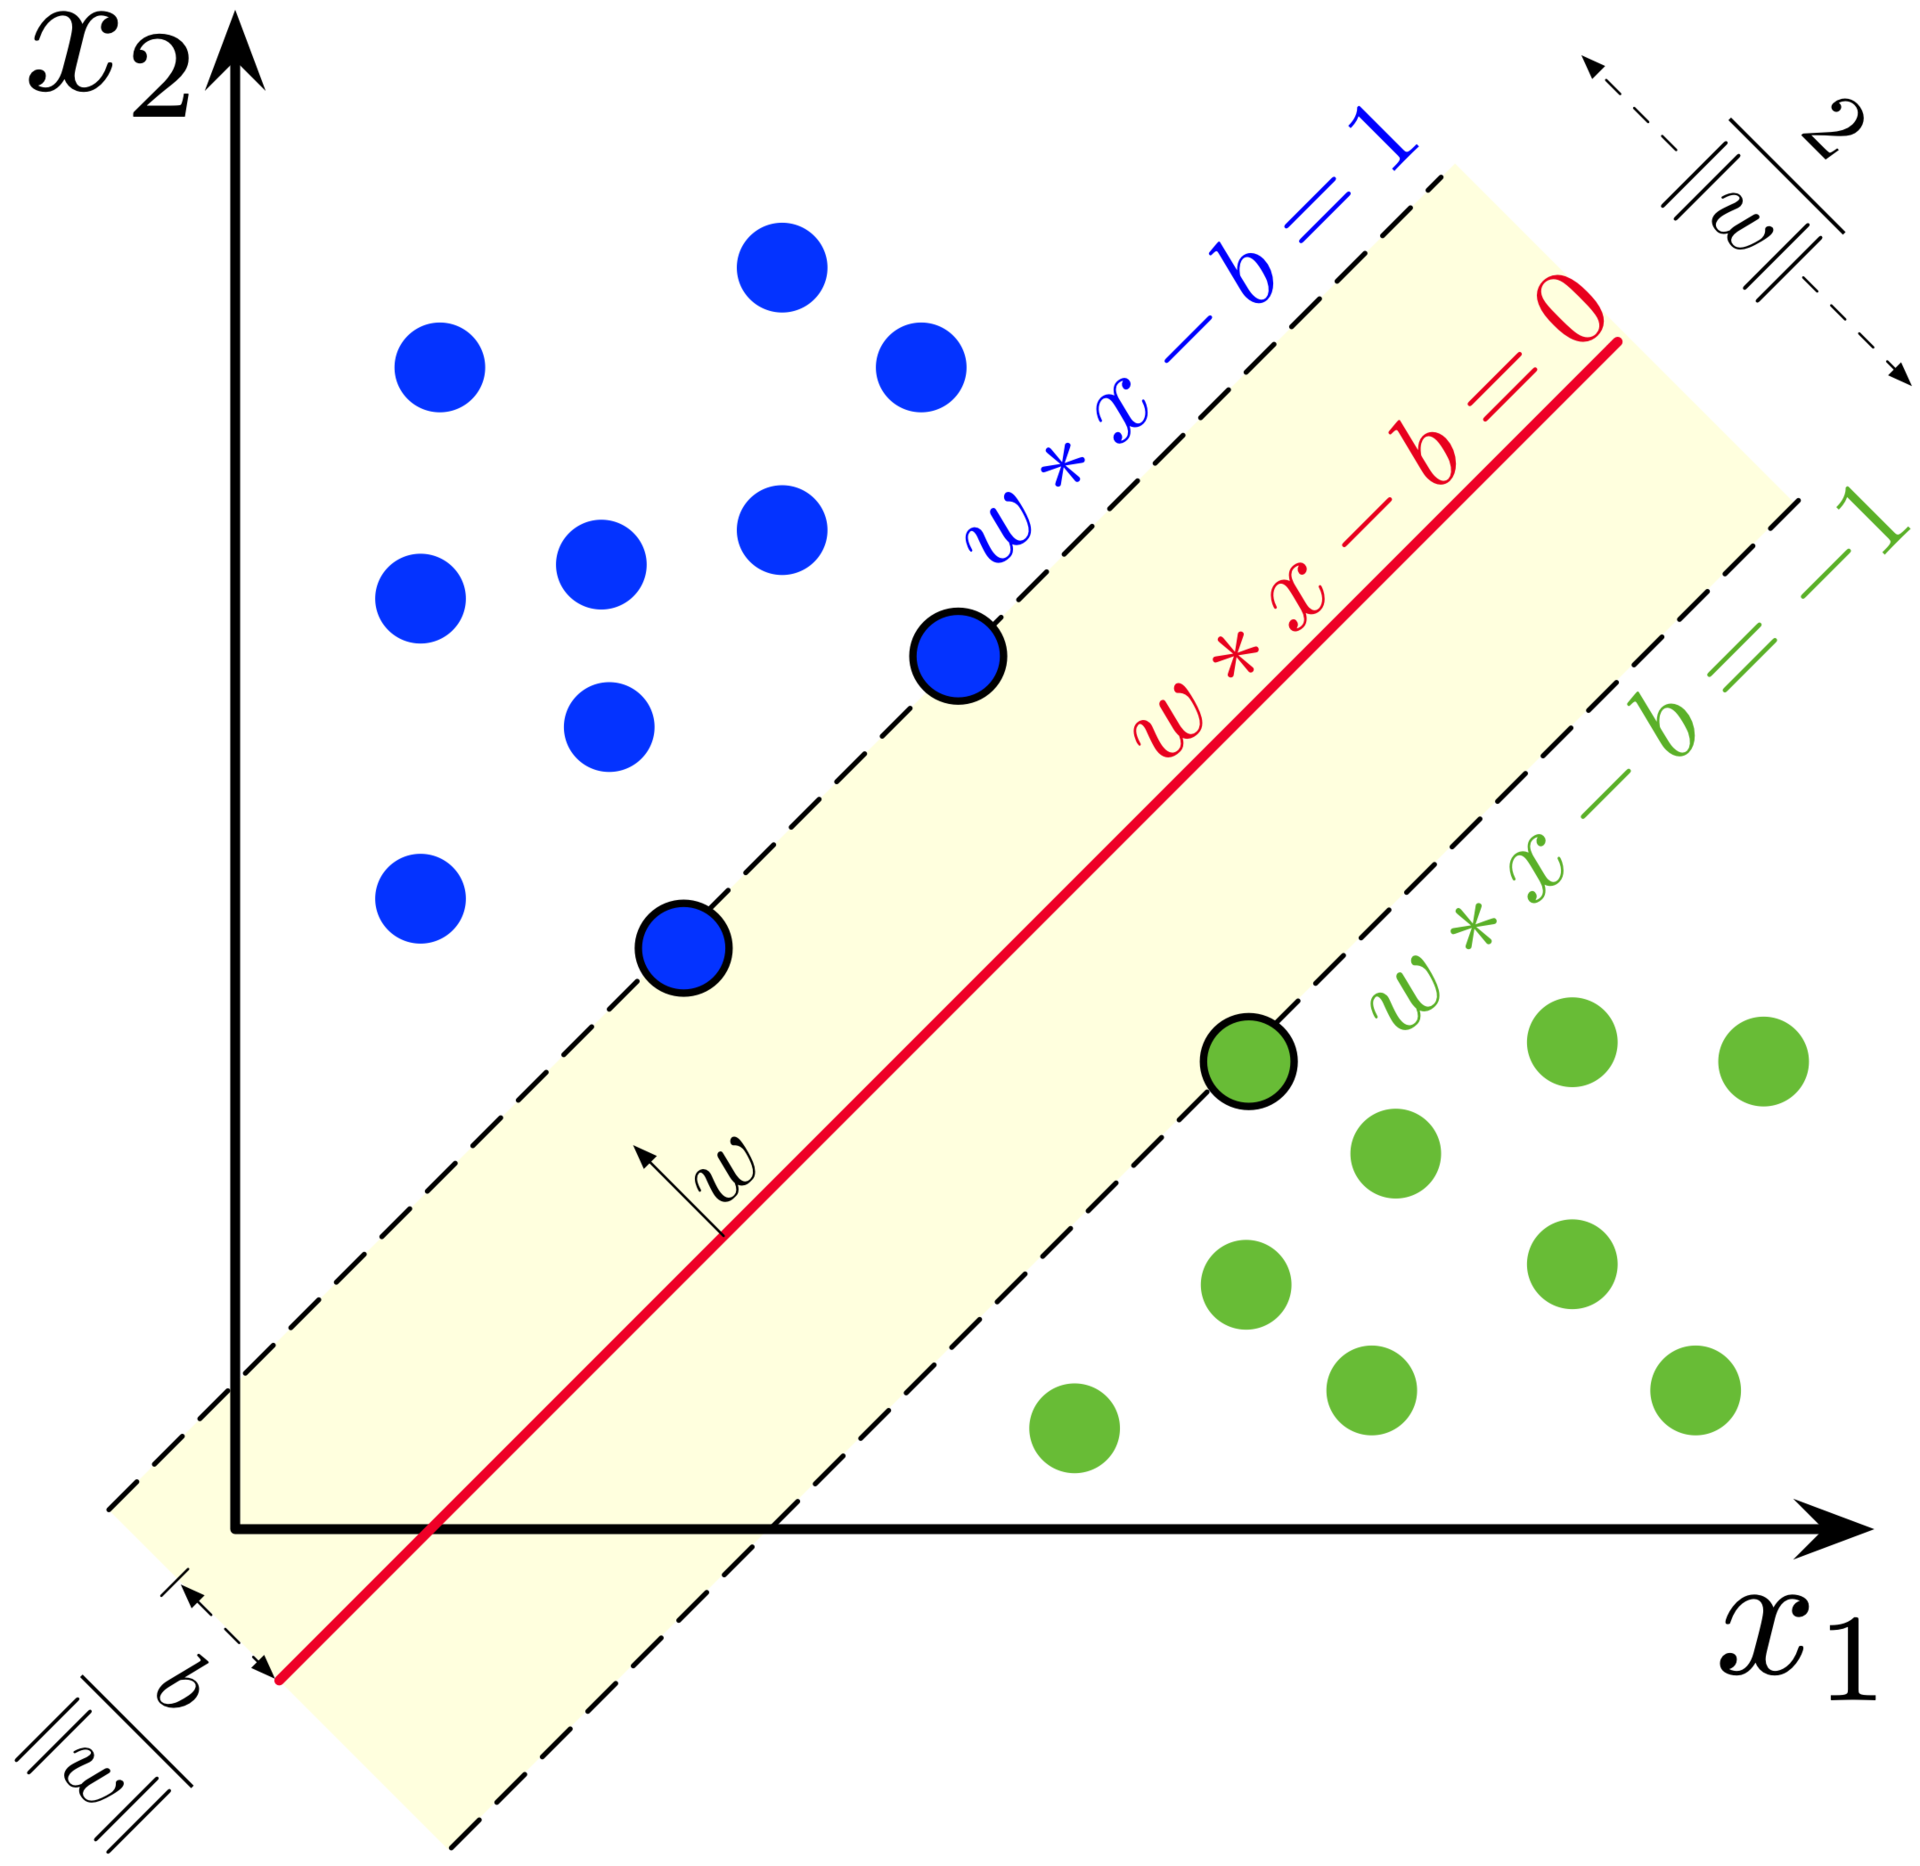
\includegraphics[width=0.45\linewidth]{/Users/JoseRomano/Documents/Tese/bca-thesis/Chapters/Figures/SVM.png}
          \caption{Visualization of a Support Vector Machine (SVM) classifier. The red line represents the optimal hyperplane that separates two classes (blue and green points), while the dashed lines indicate the margins.}
        \end{figure}
\end{itemize}

In order to evaluate a model, performance metrics are used to assess how well
it performs across different dimensions, such as accuracy, relevance, and
sensitivity to different classes. These metrics provide quantitative insight
into the strengths and limitations of a classification algorithm, allowing
researchers and practitioners to make informed decisions when comparing models
or tuning parameters. Evaluating models using multiple metrics is especially
important in scenarios involving imbalanced datasets, where a single metric
(such as accuracy) may not provide a complete picture. The most commonly used
evaluation metrics in classification tasks, according to
\textcite{metrics_models_yaseen2021}, are:

\begin{enumerate}
  \item \textbf{Accuracy} \\
        Accuracy is the ratio of correctly predicted instances to the total number of instances. It measures the overall effectiveness of a classification model.
        \[
          \text{Accuracy} = \frac{TP + TN}{TP + TN + FP + FN}
        \]
        where:
        \begin{itemize}
          \item TP = True Positives
          \item TN = True Negatives
          \item FP = False Positives
          \item FN = False Negatives
        \end{itemize}

  \item \textbf{Precision} \\
        Precision measures the proportion of correctly predicted positive observations to the total predicted positive observations. It reflects the model’s ability to return only relevant results.
        \[
          \text{Precision} = \frac{TP}{TP + FP}
        \]

  \item \textbf{Recall (Sensitivity or True Positive Rate)} \\
        Recall is the ratio of correctly predicted positive observations to all actual positives. It indicates the model’s ability to identify all relevant cases.
        \[
          \text{Recall} = \frac{TP}{TP + FN}
        \]

  \item \textbf{F1-Score} \\
        The F1-Score is the harmonic mean of Precision and Recall, providing a balance between the two. It is particularly useful when the class distribution is imbalanced.
        \[
          \text{F1-Score} = 2 \times \frac{\text{Precision} \times \text{Recall}}{\text{Precision} + \text{Recall}}
        \]

  \item \textbf{Support} \\
        Support refers to the number of actual occurrences of each class in the dataset. While not a performance metric per se, it helps in understanding how many examples a classifier is making predictions on for each class.
\end{enumerate}

Now that we are familiar with the main concepts of classification models and
the metrics used to evaluate them, let us return to the study by Wu and Hicks
(2021) in light of these indicators. The analysis of the results, presented in
the following table, allows us to see more clearly how each algorithm performed
in the task of distinguishing between TNBC and non-TNBC, highlighting the
performance of SVM in virtually all scenarios evaluated.

\begin{table}[h!]
  \centering
  \begin{tabular}{|l|c|c|c|c|c|}
    \hline
    \textbf{Model} & \textbf{Accuracy} & \textbf{Recall} & \textbf{Precision} & \textbf{F1-score} & \textbf{Specificity} \\
    \hline
    kNN            & 0.81              & 0.76            & 0.80               & 0.78              & 0.86                 \\
    Naïve Bayes    & 0.84              & 0.81            & 0.83               & 0.82              & 0.88                 \\
    Decision Tree  & 0.88              & 0.86            & 0.87               & 0.86              & 0.89                 \\
    \textbf{SVM}   & \textbf{0.90}     & \textbf{0.87}   & \textbf{0.90}      & \textbf{0.88}     & \textbf{0.90}        \\
    \hline
  \end{tabular}
  \caption{Performance of models in classifying \gls{bc} subtypes (TNBC vs non-TNBC) based on differential gene expression.}
  \label{tab:model-performance}
\end{table}

In the complete gene set, SVM achieved 90\% accuracy, 87\% recall, and 90\%
specificity - metrics that indicate, respectively, the proportion of correct
classifications, the ability to correctly identify TNBC cases, and the ability
to avoid false positives. The analysis of these metrics is essential to
correctly interpret the results in a clinical context, where the consequences
of classification errors can be significant.

To validate the robustness of the differentially expressed gene selection
approach, the authors compared it with other classic feature selection methods,
such as \textit{SVM-RFE} (an iterative technique that removes the least
relevant features based on \textit{SVM} weights), \textit{Relief} (which
weights features based on their correlation with the class), \textit{ARCO}, and
\textit{mRMR} (which maximizes relevance and minimizes redundancy between
variables). Even so, the model based on differential expression and
\textit{SVM} demonstrated better performance in most cases, confirming the
soundness of the strategy adopted.

The study further deepened the analysis of feature importance by evaluating the
performance of models with different sizes of gene subsets, from the initial
5,502 to only 16 genes. Interestingly, \textit{SVM} performance remained high
even with reduced sets, achieving the best results with 256 genes. This
stability suggests that discriminative information is concentrated in a small
subset of features, which is relevant for scenarios with a low number of
samples and a large number of features, as we have in this dissertation, and
quite positive because:

\begin{itemize}
  \item it allows molecular tests to be cheaper and faster since fewer genes are
        needed;
  \item it makes models easier to validate in a clinical setting since it is simpler to
        obtain quality samples with few targets;
  \item greater interpretability for physicians.
\end{itemize}

The analysis of the two studies presented here allows us to consolidate a
fundamental idea for this dissertation: \gls{ml} and \gls{dl} algorithms
demonstrate a remarkable ability to \textbf{classify different types of cancer
  based on complex data}, whether imaging or molecular. From deep neural networks
applied to dermatological imaging to discriminative algorithms used to analyze
gene expression, these models have proven to be effective tools for supporting
clinical decisions, sometimes proving superior to human experts. More than just
efficient classifiers, these systems have also proven to be interpretable,
robust, and applicable in real clinical scenarios. Both the image-based
approach \cite{ai_in_dermacancer_esteva2017} and the gene expression-based
approach \cite{bca_subtypes_with_ml_Wu_2021} have faced and overcome challenges
typical of medical practice and biomedical research: sample scarcity, high
dimensionality, and the need for models with good overall performance, but also
\textbf{confidence in the prediction of clinically critical cases}.

These findings provide the \textbf{conceptual support needed to explore a more
  specific direction}: the use of \gls{ml} models to discover and validate
\textbf{\gls{mirna} as biomarkers} in oncology. Like coding genes, \gls{mirna}
carry rich and discriminative information about the biological state of cells
and have shown promise in the stratification of tumor subtypes. The next
section addresses precisely this line of research, focusing on how ML has been
used to reveal \gls{mirna} signatures with diagnostic and prognostic value - a
foundation point for the objectives of this dissertation.

\subsection{\gls{ml} unravelling \gls{mirna} as biomarkers}
% Papers a usar: 1, 2 e 3

As previously discussed, artificial intelligence models have demonstrated
proficiency in the task of classificating tumor type, or subtype, by either
analysing clinical images, high-dimensional genomic data and other forms of
data. In this thesis, our focus is into a more specific and pertinent domain:
the identification of \gls{mirna} as biomarkers in oncological contexts through
\gls{ml} techniques. We know for a fact that \gls{mirna} are a class of small
molecules that have been demonstrated to possess a substantial regulatory
capacity over gene expression \ref{sec:microRNA}, but even though this capacity
distinguishes them as optimal candidates for utilization as molecular
biomarkers, the number of \glossary{mirna} expressed in human tissues, in
conjunction with their variability across individuals, demands the
implementation of robust computational methodologies.

In this context, \gls{ml} models have gained prominence as powerful tools for
revealing latent patterns in \gls{mirna} expression data, allowing the
identification of subsets with diagnostic, prognostic, or tumor subtype
stratification value. This research trajectory is particularly auspicious, as
it proffers more readily implementable, non-invasive methodologies that can be
substantiated within a clinical environment. That's what we are going to
explore in this section, where we we will present three papers that illustrate
different stages of this scientific effort: the first being a general reference
of the type of work that we will be analyzing giving us a glampse of how
\gls{ml} can work in this context; the second one being a more detailed
pipeline applied to the identification of \gls{mirna} as biomarkers for gastric
cancer, and lastly, the intersection of this kind of approach with
\glossary{bc}, which is the central carcinoma focus of this thesis.

\noindent\rule{\linewidth}{0.4pt}

The first example of work that we will address in this subsection focused on a
major challenge in modern oncology: “Is there a reliable and clinically
relevant molecular biomarker for the diagnosis and prognosis of gastric
cancer?” Despite growing evidence of the regulatory role of \gls{mirna} in
tumor progression and aggressiveness, their biological complexity (as already
mentioned in section \ref{sec:mirna_complexity}) makes it difficult to select
those with true clinical value from among the thousands that exist, and despite
these barriers, considering that gastric cancer has one of the lowest survival
rates in a 5 year period (between 20\% and 30\% survival rate) with a big share
due to late detection, usually when the tumor is already in a advanced stage
and metastasized. Given this scenario, the authors
\textcite{ml_gastric_Azari2023} propose a methodical and well-structured
\gls{ml}-based approach, as we can see in the workflow chart, to automate the
process of discovering these \gls{mirna} that may be biomarkers, where the
result also has added robustness so that it can be replicated in a real
clinical environment.

\begin{figure}
  \centering
  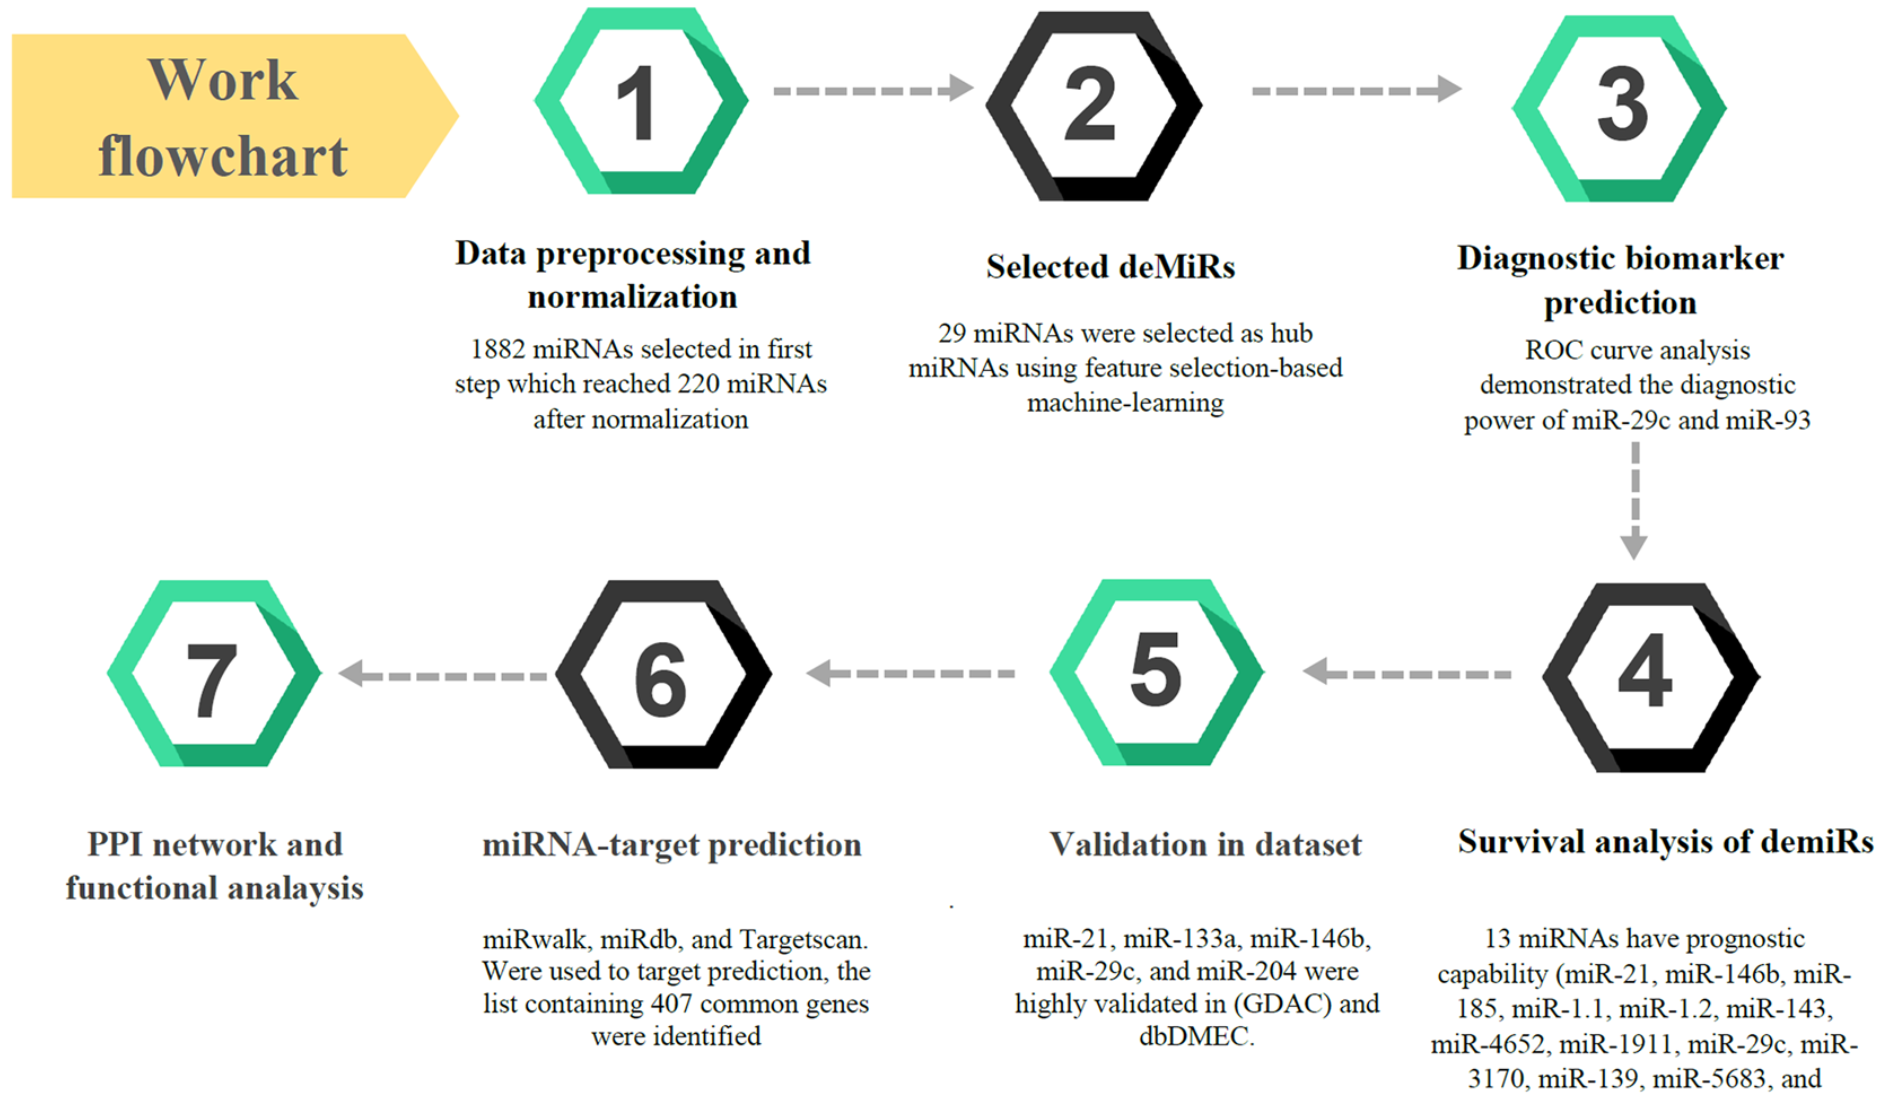
\includegraphics[width = 1.0\textwidth]{/Users/JoseRomano/Documents/Tese/bca-thesis/Chapters/Figures/workflow_gastric.png}
  \caption{Fluxogram of the methodology used in this study, including all the results obtained on each step. \cite{ml_gastric_Azari2023}}
\end{figure}

The research was based on data from 576 samples from gastric cancer patients,
collected from the TCGA repository (previously used on other studies),
including \gls{mirna} expression profiles and associated clinical information -
this clinical information includes patient characteristics such as age, gender,
among others - adding 1,882 features whose expression in a real context is not
uniform. Therefore, similar to the study on \gls{bc} subtyiping with \gls{ml},
a differential expression analysis was performed, resulting in a reduction to
only 220 of these molecular regulators (a much more acceptable and
interpretable value than the 1882 previously). Following this extensive data
preprocessing, the authors set up a classification pipeline consisting of five
classic \gls{ml} algorithms: Support Vector Machine, Random Forest, Decision
Tree, Logistic Regression, and K-Nearest Neighbors \ref{list:models} (all of
which have been discussed previously except for Random Forest, which consists
of a set of several DTs), all of which were evaluated using metrics such as
F1-score, \textit{AUC}, and confusion matrices.

\begin{table}[H]
  \centering
  \caption{Performance of the evaluated classification algorithms.}
  \label{tab:performance_azari}
  \begin{tabular}{|l|c|c|}
    \hline
    \textbf{Algorithm} & \textbf{Accuracy (\%)} & \textbf{\textit{AUC} (\%)} \\
    \hline
    DTS                & 88                     & 47.0                       \\
    Random Forest      & \textbf{93}            & 39.5                       \\
    SVM                & \textbf{93}            & \textbf{88.5}              \\
    KNN                & \textbf{93}            & 41.7                       \\
    Logistic           & \textbf{93}            & 88.0                       \\
    \hline
  \end{tabular}
\end{table}

With regard to the performance of the predictive models (as presented in table
\ref{tab:performance_azari}), the results show substantial differences between
the classifiers. Although four of the five models - all except Decision Trees -
achieved an accuracy of 93\%, the analysis of the area under the curve
(\textit{AUC}) revealed a more complex and informative picture. SVM stood out
as the most balanced model, achieving an \textit{AUC} of 88.5\%, which
indicates a strong discriminatory capacity (i.e. the model not only gets it
right often, but also assigns probabilities reliably). In contrast, models such
as KNN and RF, despite their high accuracy, obtained very low \textit{AUCs}
(41.7\% and 39.5\%, respectively), suggesting poor calibration of probabilistic
predictions and possible overfitting to the training set. The Decision Tree
(DT), with slightly lower accuracy (88\%) and an \textit{AUC} of only 47\%,
showed a more modest performance compared to the others, probably due to its
vulnerability to variance in data sets with more noise. Finally, logistic
regression also showed robust performance, with an \textit{AUC} of 88\%, very
close to that obtained by SVM. However, SVM offered better generalization or
sensitivity, justifying its selection as the final model (as already discussed
in the work by \textcite{bca_subtypes_with_ml_Wu_2021}). This analysis
highlights the importance of considering multiple metrics in model evaluation,
especially in clinical contexts, where the reliability of the assigned
probabilities - and not just the hit rate - can be decisive for a safe medical
decision.

Considering the chosen model, a processing step was performed where the most
important features were selected using a heatmap analysis, which helps to
identify patterns and the relevance of \gls{mirna} in this disease. This step
resulted in the reduction of 220 candidates to only 29 (5 of which are
significantly up-regulated and 24 considerably down-regulated - in Figure
\ref{fig:regulation_levels}), which is a very important result as it makes the
interpretation of the relationships between these potential biomarkers much
more human-friendly.

\begin{figure}
  \centering
  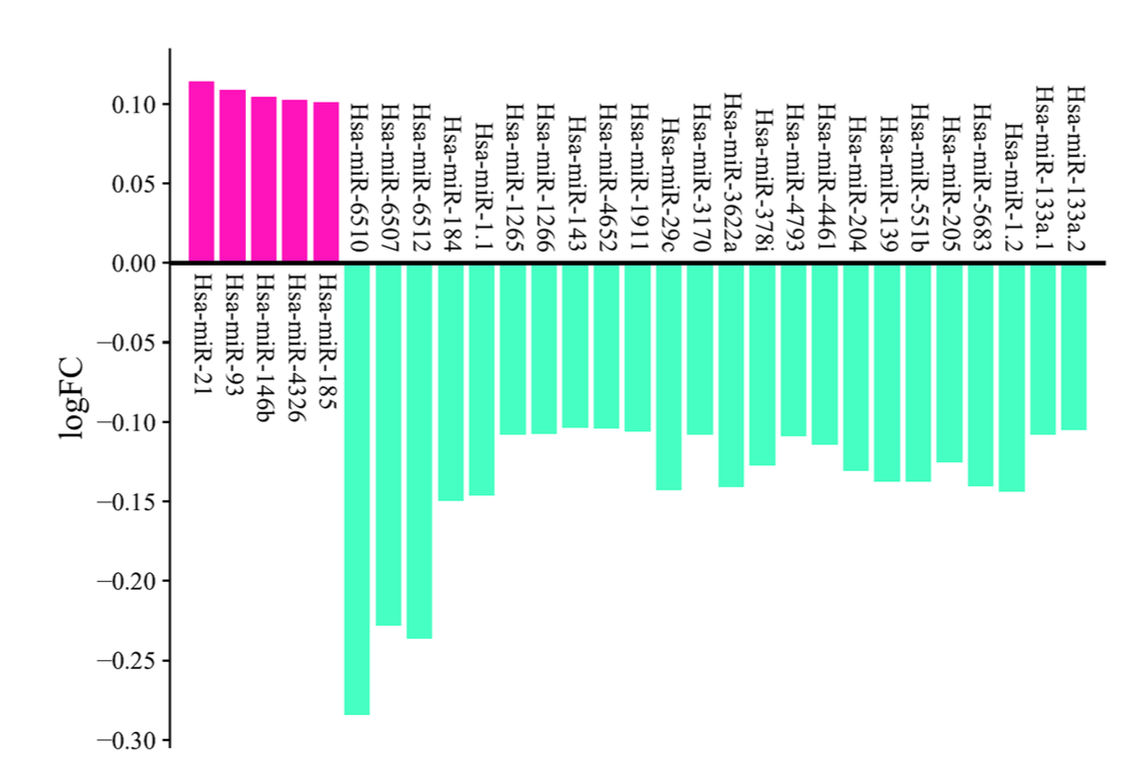
\includegraphics[width = 0.6\textwidth]{/Users/JoseRomano/Documents/Tese/bca-thesis/Chapters/Figures/up-down-regulation-azari.png}
  \caption{
    Differential regulation levels of the 29 \gls{mirna} selected by the SVM model in the study by \textcite{ml_gastric_Azari2023}. Positive logFC (log fold-change) values indicate overexpressed \gls{mirna} (magenta) and negative values indicate underexpressed \gls{mirna} (green) in gastric cancer samples compared to healthy tissue.}
  \label{fig:regulation_levels}
\end{figure}

After identifying 29 candidate \gls{mirna} from the reduced set of 220
\gls{mirna}, the authors proceeded to a validation and refinement stage. This
phase aimed to ensure that the selected \gls{mirna} not only stood out
statistically in the training set but also maintained biological relevance and
predictive robustness in independent scenarios. To this end, cross-validation
was performed in external databases, such as the Global Data Assembly Centres
(GDAC) and dbDMEC, which aggregate information from public repositories such as
GEO, SRA, ArrayExpress, and TCGA. This process allowed us to identify five
\gls{mirna} with consistent differential expression in multiple cancer
contexts: hsa-miR-21, hsa-miR-133a, hsa-miR-146b, hsa-miR-29c, and hsa-miR-204,
all classified as “highly validated". These markers stood out for their high
ability to discriminate between healthy and pathological states and, at the
same time, predict patient prognosis, positioning themselves as a potential
tool of clinical value for the diagnosis and monitoring of gastric cancer.
Complementarily, ROC curve analyses were conducted to estimate the diagnostic
potential of each \gls{mirna}, as well as survival analyses to assess their
prognostic value, demonstrating a a better indicator performance when combining
two \gls{mirna} together (Figure \ref{fig:roc_azari}).

However, the study's major revelation is not limited to predictive capacity.
The final set of four/five selected \gls{mirna} (hsa-miR-21, hsa-miR-133a,
hsa-miR-146b, and hsa-miR-29c + hsa-miR-204) underwent additional functional
validation, which allowed the identification of the genes targeted by the
selected microRNA. This identification was achieved by constructing a protein
interaction network (PPI) (Figure \ref{fig:mirna_to_gene}). This phase
confirmed that the genes regulated by these \gls{mirna} are involved in
processes essential to gastric carcinogenesis, such as Wnt signaling or
epigenetic regulation. hsa-miR-29c stood out above all for its simultaneous
predictive value for diagnosis and prognosis, reinforcing its clinical
potential as a dual biomarker.

\begin{figure}[htbp]
  \centering
  \begin{subfigure}[b]{0.49\textwidth}
    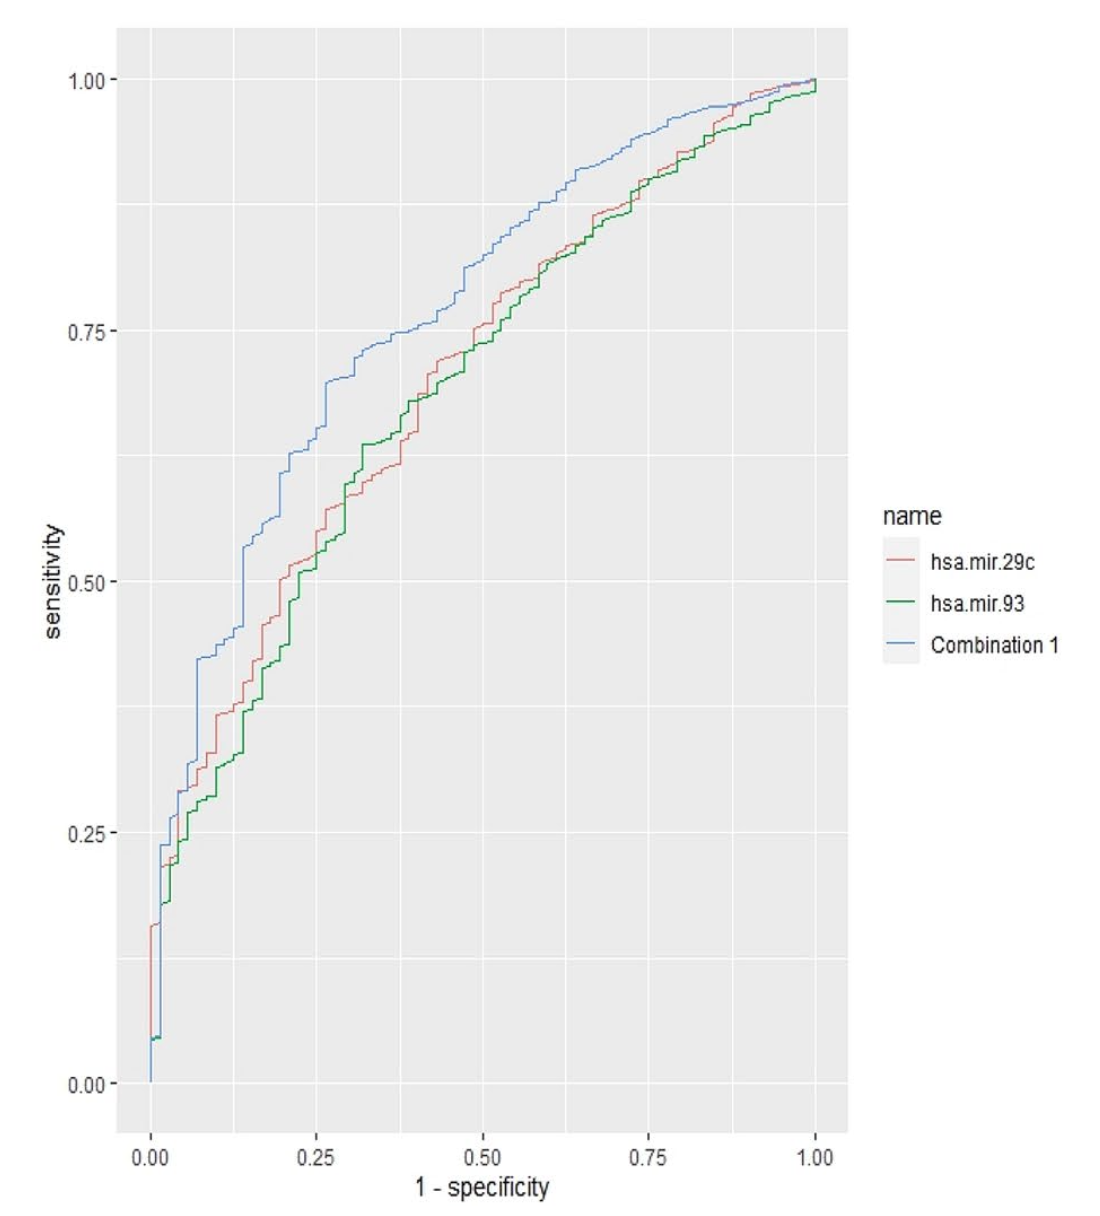
\includegraphics[width =\textwidth]{/Users/JoseRomano/Documents/Tese/bca-thesis/Chapters/Figures/roc_azari.png}
    \caption{}
    \label{fig:roc_azari}
  \end{subfigure}
  \hfill
  \begin{subfigure}[b]{0.45\textwidth}
    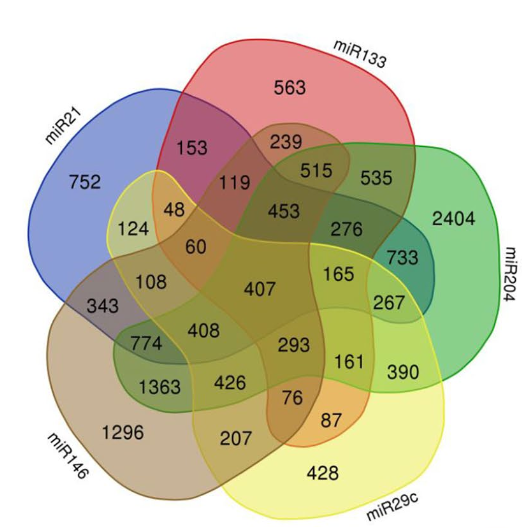
\includegraphics[width =\textwidth]{/Users/JoseRomano/Documents/Tese/bca-thesis/Chapters/Figures/mirna_to_gene.png}
    \caption{}
    \label{fig:mirna_to_gene}
  \end{subfigure}
  \caption{(a) ROC curve comparing the diagnostic performance of individual
    microRNAs (hsa-miR-29c and hsa-miR-93) versus their combination. The combined
    model (blue) shows superior sensitivity and specificity, indicating improved
    discriminative power for gastric cancer classification. \\
    \newline
    (b) Venn diagram
    illustrating the overlap of predicted gene targets
    among five microRNAs (miR-21, miR-133, miR-204, miR-146, and miR-29c)
    associated with gastric cancer. The central overlap of 426 genes indicates
    shared regulatory targets across all five \gls{mirna}, suggesting
    involvement in common biological pathways. Unique and partially overlapping
    regions highlight miRNA-specific and combinatorial regulatory potential,
    supporting their relevance as diagnostic and prognostic biomarkers.}
  \label{fig:combined}
\end{figure}

It's now a fact that identifying \gls{mirna} that are promising biomarkers
requires a study involving several different stages, as we saw in the study by
\textcite{ml_gastric_Azari2023}, but the impact of the results obtained is of
such magnitude that it fully justifies this complexity. From statistical
pre-selection to functional and biological validation, each phase contributed
to ensuring that the identified \gls{mirna} were not only statistically
relevant but also biologically plausible and clinically actionable. The final
panel of four \gls{mirna}, validated at multiple levels, represents a concrete
contribution to the construction of more accessible, interpretable, and
potentially applicable diagnostic and prognostic tools in clinical practice.
This work not only illustrates the power of \gls{ml} in biomarker discovery,
but also establishes a solid methodological foundation that can be replicated
and adapted to other diseases - including \gls{bc}, the focus of this
dissertation.

\noindent\rule{\linewidth}{0.4pt}

If the previous study demonstrated how it is possible, through a robust machine
learning pipeline, to reduce thousands of candidate \gls{mirna} to a small
panel with proven clinical potential for gastric cancer, it is natural to ask:
is it possible to apply the same principles of statistical selection,
biological validation, and predictive modeling in a context closer to the focus
of this dissertation, namely \glossary{bc}? This is precisely the proposal of
the work of \textcite{val_of_mirna_as_biomarker_Rehman_2019}, which starts from
a clinically identified set of \gls{mirna} associated with \gls{bc} and seeks,
with the aid of \gls{ml} algorithms, not only to validate their relevance, but
also to build classifiers capable of distinguishing between healthy and
cancerous tissue with high accuracy. This study introduces a perspective that
complements that of the previous work: while \textcite{ml_gastric_Azari2023}
take an exploratory approach to biomarker discovery, this new work focuses on
the next step: the verification and validation of already known \gls{mirna}
\ref{tab:clinically_verified}, assessing the extent to which they are, in fact,
discriminative and clinically actionable. It is this transition, from discovery
to validation and based on the workflow chart used in this study
\ref{fig:workflow_val}, that we will analyze in detail in the following
paragraphs.

\begin{figure}
  \centering
  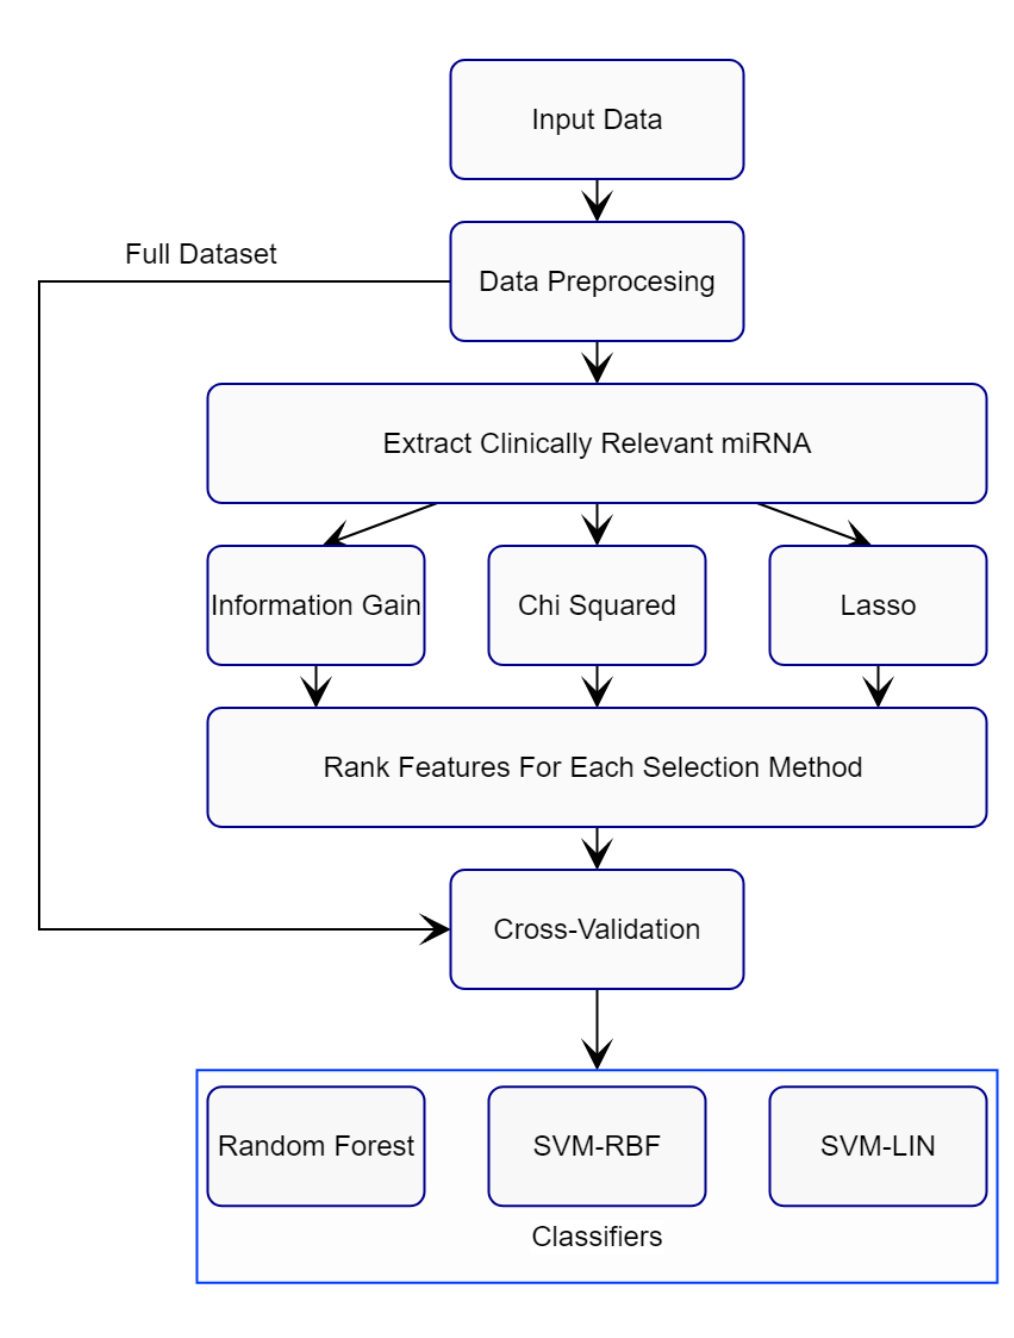
\includegraphics[width = 0.6\textwidth]{/Users/JoseRomano/Documents/Tese/bca-thesis/Chapters/Figures/pipeline_validation_mirna.png}
  \caption{Workflow chart used in the following study.}
  \label{fig:workflow_val}
\end{figure}

\begin{table}[h!]
  \centering
  \caption{List of miRNAs clinically verified.}
  \begin{tabular}{llll}
    \toprule
    \multicolumn{4}{c}{\textbf{miRNA} \cite{clinically_important_mirnas}} \\
    \midrule
    hsa-mir-10b    & hsa-let-7d   & hsa-mir-206  & hsa-mir-34a            \\
    hsa-mir-125b-1 & hsa-let-7f-1 & hsa-mir-17   & hsa-mir-27b            \\
    hsa-mir-145    & hsa-let-7f-2 & hsa-mir-335  & hsa-mir-126            \\
    hsa-mir-21     & hsa-mir-206  & hsa-mir-373  & hsa-mir-101-1          \\
    hsa-mir-125a   & hsa-mir-30a  & hsa-mir-520c & hsa-mir-101-2          \\
    hsa-mir-17     & hsa-mir-30b  & hsa-mir-27a  & hsa-mir-146a           \\
    hsa-mir-125b-2 & hsa-mir-203a & hsa-mir-221  & hsa-mir-146b           \\
    hsa-let-7a-2   & hsa-mir-203b & hsa-mir-222  & hsa-mir-205            \\
    hsa-let-7a-3   & hsa-mir-213  & hsa-mir-200c &                        \\
    hsa-let-7c     & hsa-mir-155  & hsa-mir-31   &                        \\
    \bottomrule
    \label{tab:clinically_verified}
  \end{tabular}
\end{table}

The study conducted by \textcite{val_of_mirna_as_biomarker_Rehman_2019} focuses
on the validation of a set of \gls{mirna} previously identified as clinically
relevant for \gls{bc}, using a \gls{ml} approach. Unlike exploratory
methodologies, this work starts from a list of already established candidates
and seeks to assess which of these regulatory molecules actually have robust
discriminatory potential to distinguish between healthy and tumor tissues. To
this end, the authors used a dataset composed of 1207 samples from breast
cancer patients, containing expression profiles of 1881 \gls{mirna}, obtained
from the TCGA-BRCA repository, where these were already normalized and
associated with clinical labels in order to distinguish between healthy and
tumor tissue. In addition, the normal and tumor classes are well balanced,
which helps mitigate biases in the classification models, reinforcing the
reliability of the performance evaluation metrics. However, this high
dimensionality of 1881 features required an initial feature cleaning step
(which includes the removal of null values, for example) in order to reduce the
risk of overfitting and ensure that the models do not learn patterns with
induced noise based solely on the most informative \gls{mirna}. This cleaning
left 1626 features, from which the authors, based on previous studies,
handpicked those with the most potential to discriminate \gls{bc}, resulting in
a reduced list of 36 \gls{mirna}. Three different methods, all complementary to
each other, were used for this feature selection:

\begin{enumerate} [label=(\alph*)]
  \item \textit{Information Gain} - a concept from information theory, consists of reducing
        uncertainty (entropy) by dividing the data based on a given attribute. The
        greater the information gain, the better that attribute is for classifying the
        data. \label{item:ig}

        \begin{figure}[h!]
          \centering
          \begin{subfigure}[b]{0.8\textwidth}
            \[
              E(S) = \sum_{i=1}^{c} -p_i \log_2 p_i
            \]
            \caption{}

          \end{subfigure}

          \hfill

          \begin{subfigure}[b]{0.8\textwidth}
            \[
              \text{Information Gain} = \text{Entropy(before)} - \sum_{j=1}^{K} \text{Entropy}(j, \text{after})
            \]
            \caption{}

          \end{subfigure}

          \caption{(a) Entropy formula. (b) Information Gain formula.}
        \end{figure}

  \item \textit{Chi-Squared} - the objective of this statistical method is to
        assess whether there is a relationship between a feature and the target
        variable. If this is verified, then it means that this feature is potentially
        useful for the model. \label{item:qui}

        \label{item:qui}

        \[
          \chi^2 = \sum \frac{(O - E)^2}{E}
        \]

        \begin{itemize}[label=--]
          \item $O$: observed frequency.
          \item $E$: expected frequency
        \end{itemize}

  \item \textit{LASSO} - this technique starts with a simple linear
        regression and during training automatically chooses the most
        important variables, eliminating irrelevant ones by forcing their
        coefficients to zero. All of this works with a mechanism that penalizes
        irrelevant features during training \cite{lasso_paper}.

        \label{item:lasso}

\end{enumerate}

Now, with these 36 \gls{mirna}, the authors moved on to the predictive modeling
phase, testing the effectiveness of different classifiers with progressively
smaller subsets of \gls{mirna}. Three main classification algorithms were used
(Support Vector Machine with linear kernel, SVM with RBF kernel, and Random
Forest) evaluated according to several relevant metrics: accuracy, F1-score,
sensitivity, specificity, and AUC. Validation was conducted using 10-fold
cross-validation, ensuring the reliability of the results.

\begin{table}[h!]
  \centering
  \caption{Performance Metrics across different thresholds of miRNA Features (3, 5, 10).}
  \begin{tabular}{llcccc}
    \toprule
    \textbf{Classifier} & \textbf{Method} & \textbf{Accuracy} & \textbf{Sensitivity} & \textbf{Specificity} & \textbf{AUC} \\
    \midrule
    \multirow{10}{*}{RF}
                        &                 & 0.996             & 1.000                & 0.952                & 0.999        \\
                        & IG-10           & 0.995             & 0.998                & 0.962                & 0.996        \\
                        & IG-5            & 0.996             & 0.997                & 0.977                & 0.998        \\
                        & IG-3            & 0.997             & 0.997                & 0.990                & 0.999        \\
                        & CHI2-10         & 0.995             & 0.999                & 0.952                & 0.995        \\
                        & CHI2-5          & 0.996             & 0.999                & 0.979                & 0.996        \\
                        & CHI2-3          & 0.996             & 0.997                & 0.981                & 0.999        \\
                        & LASS-10         & 0.996             & 0.998                & 0.971                & 0.997        \\
                        & LASS-5          & 0.995             & 0.997                & 0.965                & 0.998        \\
                        & LASS-3          & 0.994             & 0.997                & 0.962                & 0.999        \\

    \midrule
    \multirow{10}{*}{SVM-RBF}
                        &                 & 0.989             & 1.000                & 0.875                & 0.938        \\
                        & IG-10           & 0.994             & 0.998                & 0.952                & 0.995        \\
                        & IG-5            & 0.996             & 1.000                & 0.990                & 0.985        \\
                        & IG-3            & 0.998             & 0.998                & 0.990                & 0.980        \\
                        & CHI2-10         & 0.994             & 0.999                & 0.951                & 0.995        \\
                        & CHI2-5          & 0.996             & 0.998                & 0.983                & 0.993        \\
                        & CHI2-3          & 0.998             & 0.999                & 0.990                & 0.980        \\
                        & LASS-10         & 0.995             & 0.998                & 0.962                & 0.996        \\
                        & LASS-5          & 0.995             & 0.999                & 0.974                & 0.985        \\
                        & LASS-3          & 0.996             & 0.999                & 0.962                & 0.980        \\

    \midrule
    \multirow{10}{*}{SVM}
                        &                 & 0.997             & 0.999                & 0.971                & 0.985        \\
                        & IG-10           & 0.997             & 0.999                & 0.971                & 0.997        \\
                        & IG-5            & 0.997             & 0.999                & 0.985                & 0.989        \\
                        & IG-3            & 0.998             & 0.999                & 0.990                & 0.981        \\
                        & CHI2-10         & 0.997             & 0.999                & 0.971                & 0.997        \\
                        & CHI2-5          & 0.996             & 1.000                & 0.088                & 0.987        \\
                        & CHI2-3          & 0.998             & 0.999                & 0.990                & 0.991        \\
                        & LASS-10         & 0.994             & 0.997                & 0.962                & 0.996        \\
                        & LASS-5          & 0.995             & 0.999                & 0.956                & 0.993        \\
                        & LASS-3          & 0.997             & 1.000                & 0.962                & 0.981        \\

    \bottomrule
  \end{tabular}
\end{table}

One of the most relevant results of this study was the finding that the use of
only three highly informative \gls{mirna} could support high-quality
classifications, with performance comparable (or superior) to that obtained
with the complete set of 1881 \gls{mirna}. This has significant practical
implications, as it makes the models simpler, more interpretable, and
potentially easier to translate into a clinical context. Although the overall
accuracy is very high in all scenarios (often above 99\%), the authors point
out that this metric can be misleading in an unbalanced dataset. For this
reason, they placed particular emphasis on the analysis of sensitivity (recall)
and specificity,essential metrics in the healthcare context, where the correct
identification of patients (avoiding false negatives) and non-patients
(avoiding false positives) is critical.

The analysis of the results shows that sensitivity remained consistently high
in all models (in many cases above 0.99), reflecting the strong ability of the
classifiers to correctly identify tumor samples. Specificity, in turn, showed
clear improvements after feature selection, rising from more modest values
(such as 0.875 in SVM-RBF without selection) to levels above 0.98 in scenarios
with only three selected \gls{mirna} (e.g., IG-3 and CHI2-3 with SVM-RBF). This
improvement reveals that reducing dimensionality helped eliminate noise and
avoid misclassifying healthy samples as tumorous. Additionally, the AUC metric
remained consistently high, with values close to or even equal to 1.00,
reinforcing the robustness of the classifiers even in scenarios with a reduced
number of variables. The results also show that the three feature selection
methods (as seen in \ref{item:ig} , \ref{item:qui} and \ref{item:lasso}) led to
very similar performances, with no clear advantage of one over the others.

The results obtained in the two studies analyzed in this subsection clearly
demonstrate the central role that \gls{mirna} can play in the future of cancer
diagnosis. From the discovery of new candidates through exploratory pipelines
based on \gls{ml}, as illustrated in the work of
\textcite{ml_gastric_Azari2023}, to the rigorous validation of \gls{mirna}
previously identified as clinically relevant, as presented in
\textcite{val_of_mirna_as_biomarker_Rehman_2019}, these small molecular
regulators consistently prove to be strong indicators of tumor presence and
progression. The ability to reduce thousands of candidates to a small panel of
reliable biomarkers with clinical applicability, without compromising
predictive performance, represents a significant step toward more accessible,
non-invasive, and interpretable diagnostic tools. These findings reinforce the
fundamental premise of this dissertation: \gls{ml} models, when properly
designed and validated, can effectively exploit the complexity of \gls{mirna}
expression profiles, not only to detect cancer, but also to support more
specific tasks such as tumor subtype stratification, with real potential for
clinical translation.

\subsection{Comparison with thesis approach}

The analysis of the studies presented throughout this chapter allows us not
only to understand the state of the art in the use of \gls{ml} algorithms for
biomarker identification, but also how these computational resources can become
key elements in the classification of tumor masses, directly outlining some
possible paths for this thesis.

One of the first aspects to highlight is the \textbf{importance of differential
  expression analysis as an initial step in feature selection}. This approach was
common to several of the studies analyzed, namely
\textcite{bca_subtypes_with_ml_Wu_2021} and \textcite{ml_gastric_Azari2023},
and proved effective in reducing dimensionality in scenarios with high feature
density, such as miRNA expression data. This strategy allows the analysis to
focus on more informative subsets, reducing the risk of overfitting and making
the models more robust. In addition, the studies mentioned demonstrate that
this initial selection can (and should) be complemented with additional
computational methods. Techniques such as LASSO regression, Information Gain,
Chi-Squared, and Recursive Feature Elimination (RFE) have been explored in
different papers and show that combining statistical approaches with
model-based methods increases the probability of finding truly discriminative
features. This idea will be incorporated into the pipeline developed in this
thesis, with the aim of building more reliable and interpretable models.

Another valuable methodological element drawn from the analyzed works is the
\textbf{rigorous validation of the identified models and biomarkers}, either
through internal cross-validation or through the use of external data. The
study by \textcite{ml_gastric_Azari2023}, for example, stands out for having
validated miRNA candidates in several public repositories such as GEO, dbDMEC,
and GDAC. This type of cross-validation with other sources, even if partial,
\textbf{gives greater solidity and generalization to the results obtained}, a
key aspect that will be taken into account in the structure of this
dissertation, with the consideration of robust validation strategies. Regarding
the \textbf{origin of the data}, the reviewed studies reinforce the relevance
of using \textbf{The Cancer Genome Atlas (TCGA)} repository as a reliable,
comprehensive, and widely used data source in similar studies. This will also
be the base repository for this study, ensuring comparability with previous
studies and data quality.

It is also important to mention that both sutides showed that \textbf{the
  performance of the models does not necessarily depend on all available
  features}. On the contrary, several models have shown excellent performance
with only a fraction of the input data (such as subsets of 3 to 10 \gls{mirna})
highlighting the feasibility of building simpler, more interpretable, and
economically applicable models in a clinical context. The possibility of
finding a small group of \gls{mirna} that would have the same performance as
using all of them is the real breakthrough of a thesis like this, since it
would open doors to more affordable testing, leading to more prevention tests
and the possibility of earlier detection of these malignous cells.

Finally, the workflow diagrams proposed in the reference studies - with special
emphasis on that of \textcite{ml_gastric_Azari2023} - offer a clear,
sequential, and methodologically rigorous visual representation of all the
steps involved in the discovery and validation of molecular biomarkers using
\gls{ml}. These flowcharts not only facilitate understanding of the process,
but also help to ensure the reproducibility of studies and effective
communication of methods between researchers. In the particular case of this
dissertation, the structure presented in these works serves as direct
inspiration for the design of the pipeline that will be implemented here,
covering all critical phases: from data acquisition and pre-processing, through
careful feature selection and predictive modeling, to internal statistical
validation and model performance analysis. This systematic approach ensures
alignment with best practices in the literature and maximizes the translational
potential of the results obtained.

In short, the literature review allows us to consolidate a solid methodological
basis, anchored in studies that have demonstrated the effectiveness of machine
learning in the discovery and validation of molecular biomarkers. From this
evidence, it is clear that well-structured approaches such as combining
differential expression analysis, careful feature selection, and rigorous
validation offer a promising path to building robust and clinically relevant
predictive models. This accumulated knowledge will now be adapted and applied
to the specific context of this dissertation, which seeks to identify miRNA
signatures with discriminatory power for the classification of breast cancer
subtypes. The next chapter describes in detail how this approach will be
implemented.

% \subsection{Other relevant work}
% HERE: applying ml in diagnosis and prognosis + ai in oncological nanomedicine
% Papers a usar: 6,8,5,7

% \subsection{Conclusion}